\section{Complex Analysis}

\begin{center}
    Notes from \textbf{Math 555: Introduction to Complex Variables}

    Taken at University of Michigan, Winter 2026

    using \textit{Complex Analysis}, by Lars Ahlfors
\end{center}

\subsection{Complex Numbers}
%%% Algebra of complex numbers, Geometry of complex numbers

An initial motivation for complex numbers is in solution to equations such as $x^2+1=0$. No real number satisfies this equation, so it seems natural to introduce a number $i$ such that $i^2=-1$, and therefore $\pm i$ satisfies this equation. It also seems natural to extend the typical rules of arithmetic from the real numbers to also apply to the complex numbers. A \textit{complex number} $z$ has the form $z=a+ib$, where $a,b\in\mathbb{R}$. Note that $z$ has a real part, with $\operatorname{Re}(z) = a$, and an imaginary part, with $\operatorname{Im}(z)=b$.

The complex numbers can be viewed as $\mathbb{R}^2$ with some additional structure. In particular, a complex number $z\in \mathbb{C}$ is a vector $(a,b)\in\mathbb{R}^2$ with component-wise vector addition and the standard multiplication for real numbers. That is, for $z=a+ib$ and $w=c+id$, we have $z+w = (a+c) + i(b+d) = (a+c, b+d)$ and $zw = (a+ib)(c+id) = (ac-bd)+i(ad+bc) = (ac-bd, ad+bc)$.

Note that $\mathbb{C}$ is a \textit{field}, and in particular $\mathbb{C}$ is a \textit{field extension} of $\mathbb{R}$. That is, the real line can be viewed as a subset of $\mathbb{C}$. Namely, the set $\{z\in\mathbb{C}\mid \operatorname{Im}(z)=0\}$ is precisely the real number line. Because $\mathbb{C}$ is a field extension of $\mathbb{R}$, it inherits the usual rules for addition, subtraction, multiplication, and division. That is, we have the associative, commutative, and distributive laws, and we have the neutral elements $0$ and $1$ under addition and multiplication respectively.

Some notation for complex numbers will now be introduced. Let $z=a+ib$ be a complex number. The \textit{complex conjugate} of $z$, denoted $\overline{z}$, is given by \[\overline{z}:=a-ib\] Suppose $w$ is another complex number. Then, the following properties hold: \[\overline{w+z} = \overline{w}+\overline{z}\tag{1}\] 
\[\overline{wz} = \overline{w}\cdot\overline{z}\tag{2}\] 
\[\overline{(w/z)} = \overline{w} / \overline{z}\tag{3}\]

Property (3) follows naturally from property (2). A proof is provided for (1) and (2). \begin{proof}
    Let $w=a+ib$, $z=x+iy$. Then, we have that \begin{eqnarray*}
        \overline{w+z} &=& \overline{a+ib+x+iy}\\
        &=& \overline{(a+x) + i(b+y)}\\
        &=& (a+x) - i(b+y)\\
        &=& (a-ib) + (x-iy)\\
        &=& \overline{w} + \overline{z}
    \end{eqnarray*} Similarly, we have that \begin{eqnarray*}
        \overline{wz} &=& \overline{(a+ib)(x+iy)}\\
        &=& \overline{(ax-by)+i(ay+bx)}\\
        &=& (ax-by) - i(ay+bx)\\
        &=& ax -iay -ibx -by\\
        &=& (a-ib)(x-iy)\\
        &=& \overline{w}\cdot\overline{z}
    \end{eqnarray*}
\end{proof}

The \textit{modulus} of $z$, denoted $|z|$ and effectively representing the norm of $z$, is computed by the familiar Euclidean metric on $\mathbb{R}^2$. The modulus can be equivalently written in terms of the complex conjugate of $z$: \[|z|:=\sqrt{\operatorname{Re}(z)^2+\operatorname{Im}(z)^2} = \sqrt{\overline{z}z} \geq 0\] Note that this implies that $\overline{z}z\geq 0$, which is indeed the case. It can easily be shown that $|zw| = |z||w|$. In particular, this follows directly from the following relationship: \[|zw| = \sqrt{\overline{z}z\overline{w}w} = \sqrt{\overline{z}z}\sqrt{\overline{w}w} = |z||w|\] This result can extend to arbitrarily many complex numbers by induction.

\begin{shaded}
    \textbf{Geometry of the Complex Numbers}. As mentioned, a complex number $z\in\mathbb{C}$ is essentially a two-dimensional vector with some additional structure. It is natural to imagine $z$ to exist on the \textit{complex plane}, with the $x$-axis corresponding to the real part of $z$ and the $y$-axis corresponding to the imaginary part of $z$.

    In rectangular coordinates, $z=a+ib$ is simply the vector $(a,b)$. $z$ may also naturally be expressed in terms of polar coordinates; that is, there exists $r\geq 0$ and an angle $\theta\geq 0$ such that \[z=r\operatorname{cis}(\theta) := (r\cos\theta,r\sin\theta) = r\cos\theta + ir\sin\theta\] Note that $r=|z|$ uniquely, but $\theta$, which is called the \textit{argument} of $z$, is not uniquely defined; some notation for argument will now be introduced.

    The set of possible values for $\theta$ is denoted $\arg(z)$, and is precisely the set \[\arg(z) = \{\theta\in\mathbb{R}\mid z=(r\cos\theta,r\sin\theta)\}\] The \textit{principal branch} of the argument, denoted $\operatorname{Arg}(z)$, is a function $\operatorname{Arg}:\mathbb{C}\setminus\{0\}\to (-\pi,\pi]$ defined by $\operatorname{Arg}(z) = \theta_0$, where $\theta_0\in \arg(z)$ also satisfies the condition $-\pi<\theta_0\leq \pi$. Sometimes this function is defined instead on $[0,2\pi)$, in which case it will be denoted $\operatorname{HArg}$ in this context, with $\operatorname{HArg}(z)=\theta_0$ similarly producing a $\theta_0\in \arg(z)$ with the additional property that $0\leq \theta_0<2\pi$. Note that $\arg(z)$ may be expressed in terms of the principal argument, with $\arg(z) = \{\operatorname{Arg}(z)+2\pi n\mid n\in\mathbb{Z}\}$.

    The argument has the following properties:
    \[\arg(wz) = \arg(w)+\arg(z)\tag{1}\]
    \[\arg(w/z) = \arg(w)-\arg(z)\tag{2}\] These properties can be shown directly by the definition of $\operatorname{cis(z)}$ and applying trigonometric identities.
\end{shaded}

\subsection{Analysis on \texorpdfstring{$\mathbb{R}^n$}{R^n}}

Because $\mathbb{C}$ essentially has the structure of $\mathbb{R}^2$, it is beneficial to summarize some general results from analysis on $\mathbb{R}^n$, which can then be restricted to the case of $\mathbb{R}^2$ and therefore to $\mathbb{C}$. Most of these results are provided without proof because the result (or a more general form) has been shown in real analysis or topology, or the result readily generalizes from $\mathbb{R}$ or general metric spaces.

\begin{framed}
    \textbf{Sequences in} $\mathbb{R}^n$. Let $S$ be any set. A sequence in $S$ is a function $(x_n)_{n\in\mathbb{N}}:\mathbb{N}\to S$. In other words, $(x_n)_{n\in\mathbb{N}}$ assigns a value in $S$ to every natural number. Some relevant definitions are provided:
    \textbf{Definition}. Let $x\in\mathbb{R}^n$, and let $(x_n)_{n\in \mathbb{N}}$ be a sequence in $\mathbb{R}^n$.
    \vspace{-1em}
    \begin{enumerate}
        \item $x$ is a \textbf{limit point} of $(x_n)_{n\in\mathbb{N}}$ if for all $\varepsilon>0$, the set $\{n\in\mathbb{N}\mid |x_n-x|<\varepsilon\}$ is infinite.
        \item $(x_n)_{n\in\mathbb{N}}$ \textbf{converges to} $x$ if $\displaystyle\lim_{n\to\infty} |x_n-x| = 0$; in other words, $x$ is a \textbf{limit} of $(x_n)_{n\in\mathbb{N}}$ if for all $\varepsilon>0$, there exists $N\in\mathbb{N}$ such that for all $n\geq N$, $|x_n-x|<\varepsilon$.
        \item $(x_n)_{n\in\mathbb{N}}$ is \textbf{bounded} if there exists $M\in\mathbb{R}$ such that $|x_n|\leq M$ for all $n\in\mathbb{N}$.
        \item $(x_n)_{n\in\mathbb{N}}$ is \textbf{Cauchy} if for all $\varepsilon>0$, there exists $N\in \mathbb{N}$ such that for all $m,n\geq N$, $|x_m-x_n|<\varepsilon$.
    \end{enumerate}
\end{framed}
Another way to view this is as follows: $x$ is a limit point of $(x_n)_{n\in\mathbb{N}}$ if $x_n\in B_\varepsilon(x)$ for infinitely many values of $n$, and $x$ is a limit if there is some $N\in\mathbb{N}$ where $x_n\in B_\varepsilon(x)$ for all $n>N$, which is the topological definition of sequential convergence. Note that a sequence can have multiple limit points, but a sequence can have at most one (unique) in $\mathbb{R}^n$.

The two main theorems concerning sequences in $\mathbb{R}^n$ are provided without proof:

\textbf{Bolzano-Weierstrass Theorem} (in $\mathbb{R}^n$). Suppose $(x_n)_{n\in\mathbb{N}}$ is a bounded sequence in $\mathbb{R}^n$. Then, $(x_n)_{n\in\mathbb{N}}$ has a limit point.
\textbf{Completeness of $\mathbb{R}^n$}. A sequence $(x_n)_{n\in\mathbb{N}}$ is convergent if and only if it is Cauchy.

An alternate characterization relating limit points and limits is given. Let $(x_n)$ be a sequence in $\mathbb{R}^n$ and $x\in\mathbb{R}^n$.
\vspace{-1em}
\begin{enumerate}
    \item[(1)] $(x_n)$ converges to $x$ if and only if for every open neighborhood $U$ of $x$, there exists an $N\in\mathbb{N}$ such that $x_n\in U$ for all $n\geq N$.
    \item[(2)] $x$ is a limit point of $(x_n)$ if and only if there exists a subsequence $(x_{n_k})$ converging to $x$.
    \item[(3)] If $S\subseteq\mathbb{R}^n$, then $\overline{S}$ is precisely the set of points $y\in\mathbb{R}^n$ such that there exists a sequence in $S$ converging to $y$. That is, a closed set contains the limits of all its sequences.
\end{enumerate}

\begin{framed}
    \textbf{Series in $\mathbb{R}^n$}. Let $(x_n)_{n\in\mathbb{N}}$ be a sequence in $\mathbb{R}^n$. Then, the sequence of \textit{partial sums} is denoted by: \[(s_n)_{n\in\mathbb{N}}:=\sum_n x_n :=\left(\displaystyle\sum_{n=1}^N x_n\right)_{n\in\mathbb{N}}\] If $(s_n)_{n\in\mathbb{N}}$ converges to some $s\in\mathbb{R}^n$, then $s$ is called the \textbf{sum} of the series, and we write $\displaystyle\sum_{n=1}^\infty x_n :=\displaystyle\lim_{N\to\infty}\sum_{n=1}^N x_n = s$.

    $\sum_n x_n$ \textbf{converges absolutely} if $\displaystyle\sum_{n=1}^\infty |x_n|<\infty$, and $\sum_n x_n$ \textbf{converges conditionally} if $\displaystyle\sum_{n=1}^\infty|x_n| = \infty$.
\end{framed}

An example of a conditionally convergent series is given by $\sum_n (-1)^n/n$. This series converges, but $\sum_n|(-1)^n/n| = \sum_n 1/n$ which does not converge.

\textbf{Theorem}. Suppose $(x_n)$ is a sequence in $\mathbb{R}^n$ with the property that $\sum_n x_n$ is absolutely convergent. Then, the following properties hold:
\[\sum_n x_n \text{ is convergent}\tag{1}\] \[\left|\displaystyle\sum_{n=1}^\infty x_n\right|\leq \displaystyle\sum_{n=1}^\infty\left|x_n\right|\tag{2}\] Property (2) is called the "infinite triangle inequality."

Let $\rho:\mathbb{N}\to\mathbb{N}$ be a bijection. Then, the series $\sum_n x_{\rho(n)}$ is a \textit{rearrangement} of $\sum_n x_n$. The rearrangement of a series is not in general equivalent to the original series, except under the condition of absolute convergence. If $(x_n)$ is not absolutely convergent, this statement fails (in spectacular fashion):

\textbf{Riemann's Rearrangement Theorem}. Suppose $\sum_n x_n$ is a conditionally convergent series of real numbers.\\ Let $s\in \mathbb{R}\cup\{-\infty, \infty\}$. Then, there exists a bijection $\rho:\mathbb{N}\to\mathbb{N}$ such that $\displaystyle\sum_{n=1}^\infty x_{\rho(n)} = s$. There also exists a bijection $\rho$ such that $\displaystyle\sum_{n=1}^\infty x_{\rho(n)}$ does not converge to a real limit or $\pm\infty$.

\newpage
\begin{shaded}
    \textbf{Cauchy Product of Infinite Series}. Let $(w_n)$ and $(z_n)$ be sequences of complex numbers (or, therefore, real numbers). From analysis, we have that sequences can sum: \[\sum_{n=1}^\infty (w_n + z_n) = \sum_{n=1}^\infty w_n + \sum_{n=1}^\infty z_n\] which converges (or converges absolutely) if the individual series converge (or converge absolutely). The \textbf{Cauchy product} of $\sum_n z_n$ and $\sum_n w_n$ is a similar procedure, which is defined as follows: \[\sum_n \left(\sum_{i=0}^nz_iw_{n-1}\right) = \sum_n \left(\sum_{i+j=n} z_i w_j\right)\] \textbf{Theorem (Convergence of Cauchy Products)}. If $\sum_n z_n$ converges \textit{absolutely} and $\sum_n w_n$ converges, then their Cauchy product converges, and: \[\sum_{n=0}^\infty \left(\sum_{i=0}^\infty z_i w_{n-i}\right) = \sum_{n=0}^\infty z_n \sum_{n=0}^\infty w_n\]
\end{shaded}

There are several useful tests for whether a series converges or diverges; these are familiar from standard analysis, and the results extend generally from $\mathbb{R}$ to $\mathbb{R}^n$:

\begin{shaded}
    \textbf{Series Tests}. The following tests can be used to conclude whether a series converges or diverges. Let $(x_n)$ be a sequence in $\mathbb{R}^n$.
    
    \textbf{Divergence Test}. If $\sum_n x_n$ converges, then $\displaystyle\lim_{n\to\infty} x_n = 0$. Importantly, the negation is that if $\displaystyle\lim_{n\to\infty} x_n\neq 0$, then $\sum_n x_n$ does not converge.

    \textbf{Comparison Test}. If $(y_n)$ is a sequence in $\mathbb{R}^n$ such that $\sum_n y_n$ converges absolutely and $|x_n|\leq |y_n|$ for all $n\in\mathbb{N}$, then $\sum_n x_n$ converges absolutely.

    \textbf{Root Test}. If $\displaystyle\limsup_{n\to\infty} |x_n|^{1/n} < 1$, then $\sum_n x_n$ converges absolutely. If $\displaystyle\limsup_{n\to\infty} |x_n|^{1/n} > 1$, then $\sum_n x_n$ diverges.

    \textbf{Ratio Test}. Suppose $x_n\neq 0$ for all $n\in\mathbb{N}$. If $\displaystyle\limsup_{n\to\infty} \frac{|x_{n+1}|}{|x_n|}< 1$, then $\sum_n x_n$ converges absolutely. If $\displaystyle\liminf_{n\to\infty} \frac{|x_{n+1}|}{|x_n|}> 1$, then $\sum_n x_n$ diverges.
\end{shaded}

\begin{framed}
    \textbf{Compact Subsets of $\mathbb{R}^n$}. Recall from topology that a set $U\subseteq\mathbb{R}^n$ is called \textit{compact} if every cover of $U$ has a finite subcover. In $\mathbb{R}^n$, there is a more useful characterization from analysis:

    \textbf{Heine-Borel Theorem}. A subset of $\mathbb{R}^n$ is compact if and only if it is closed and bounded.

    Because sequential compactness is equivalent to compactness in Euclidean space, we also have a sequential characterization of compactness:

    \textbf{Sequential Characterization of Compactness}. A subset $U\subseteq\mathbb{R}^n$ is compact if and only if every sequence in $U$ has a convergent subsequence with limit in $U$.
\end{framed}

\newpage
The familiar $\varepsilon-\delta$ definition of convergence and continuity generalize to $\mathbb{R}^n$:

\begin{framed}
\textbf{Convergence and Continuity}. Let $S\subseteq\mathbb{R}^m$, $T\subseteq \mathbb{R}^n$, and $f:S\to T$.

\textbf{Definition of Convergence}. Let $x_0\in\overline{S}$. $f(x)$ \textbf{converges} to $L\in\mathbb{R}^n$ if for all $\varepsilon>0$, there exists $\delta>0$ such that if $x\in S$ and $0<|x-x_0|<\delta$, then $|f(x)-L| < \varepsilon$. In this $L$ is the \textit{limit} as $x\to x_0$, denoted: \[\lim_{x\to x_0,x\in S} f(x) = L\] \textbf{Definition of Continuity}. Let $x_0\in S$. $f$ is \textbf{continuous} at $x_0$ if for all $\varepsilon>0$ and all $y\in S$, there exists $\delta>0$ such that if $x\in S$ and $|x-y|<\delta$, then $|f(x)-f(y)|<\varepsilon$. This is equivalent to the statement that: \[\lim_{x\to x_0,x\in S} f(x) = f(x_0)\] \textbf{Definition of Uniform Continuity}. $f$ is \textbf{uniformly continuous} on $S$ if for all $\varepsilon>0$, there exists $\delta>0$ such that if $x,y\in S$ and $|x-y|<\delta$, then $|f(x)-f(y)|<\varepsilon$.

Note that in the definition of continuity, $\delta$ \textit{can} depend on $y$, i.e. $\delta = \delta(\varepsilon,y)$, but in the uniform continuity definition $\delta$ may \textit{not} depend on $y$, i.e. $\delta = \delta(\varepsilon)$ alone.
\end{framed}

Using the fact that for compact sets $C$, $f(C)$ is compact, the extreme value theorem can be shown: 

\textbf{Extreme Value Theorem}. Suppose $C\subseteq\mathbb{R}^n$ is a nonempty, compact set and $f:C\to\mathbb{R}$ is continuous. Then, there exist $x_m,x_M\in C$ such that $f(x_m) = \min\{f(x)\mid x\in C\}$ and $f(x_M) = \max \{f(x)\mid x\in C\}$.

In one dimension, a function $f:(a,b)\to\mathbb{R}$ is \textit{real-differentiable} at $x_0\in(a,b)$ if: \[f'(x_0) := \lim_{x\to x_0} \frac{f(x)-f(x_0)}{x-x_0} \text{ \ exists}\] This definition does not immediately generalize to higher dimensions; however, an equivalent characterization is that $f$ is differentiable if there is a line passing through $(x_0,f(x_0))$ which accurately approximates the function. Then, $f$ is \textit{real-differentiable} at $x_0$ if \[\lim_{x\to x_0} \frac{|f(x)-f(x_0) - m(x-x_0)|}{|x-x_0|} = 0\] Note that the slope $m=f'(x_0)$. This definition can be readily generalized to the $\mathbb{R}^n$ case.

\textbf{Definition of Real-Differentiability}. Let $U\subseteq \mathbb{R}^m$ be open. Let $x_0\in U$. A function $f:U\to \mathbb{R}^n$ is \textbf{real-differentiable} at $x_0$ if there exists an $m\times n$ matrix $A$ such that \[\lim_{x\to x_0} \frac{|f(x)-f(x_0)-A(x-x_0)|}{|x-x_0|} = 0\] Alternatively, we may define the error $\varepsilon(x)$ of the linear approximation, and rewrite in planar form: \[f(x) = f(x_0) + A(x-x_0) + \varepsilon(x),\text{ where }\lim_{x\to x_0}\frac{|\varepsilon(x)|}{|x-x_0|} = 0\] Note that this can equivalently be rewritten as: \[\varepsilon(x) = f(x) - f(x_0) - A(x-x_0) \implies \lim_{x\to x_0}\frac{|f(x)-f(x_0)-A(x-x_0)|}{|x-x_0|} = 0 \text{ if }f\text{ is real-differentiable}\]

The matrix $A$ is unique, and $A$ is called the \textbf{Jacobian matrix of $f$ at $x_0$}, or the \textbf{total derivative}. $A$ essentially contains the "slopes" (the derivatives) of $f$. That is, if $f$ is represented as the vector $f=(f_1,\dots, f_m)$ where $f_i:U\to\mathbb{R}$, then $a_{ij} = \displaystyle\frac{\partial f_i}{\partial x_j} \bigg\rvert_{x=x_0}$, i.e. the $ij$th entries are the partial derivatives of $f_i$ with respect to $x_j$.

Note that if $f$ is real-differentiable at $x_0$, then the partial derivatives $\partial_j f_i(x_0)$ exist. The opposite is \textbf{not} true. Additionally, the existence of partial derivatives does not guarantee a function of several variables is real-differentiable, and a function which is real-differentiable can have discontinuous partial derivatives.

\begin{shaded}
    \textbf{Sequences of Functions}. Let $S\subseteq\mathbb{R}^m$, $f:\mathbb{R}^m\to \mathbb{R}^n$, and $(f_n)_{n\in\mathbb{N}} = (f_n:S\to\mathbb{R}^n)_{n\in\mathbb{N}}$.

    \textbf{Definition (Pointwise and Uniform Convergence)}. $(f_n)_{n\in\mathbb{N}}$ is \textbf{pointwise convergent} to $f$ if for all $x\in S$, $(f_n(x))_{n\in\mathbb{N}}$ converges to $f(x)\in\mathbb{R}^n$. $f$ is \textbf{uniformly convergent} to $f$ if $\displaystyle\lim_{n\to\infty} \left(\sup_{x\in S}\left|f_n(x)-f(x)\right|\right) = 0$.

    It is useful to translate these definitions into quantifiers:

    \begin{center}
        \begin{tabular}{c|c}
            \textbf{Pointwise Convergence} & \textbf{Uniform Convergence} \\
            \hline\hline
            $\forall x\in S$ and $\forall\varepsilon>0$, &  $\forall\varepsilon>0$,\\
            $\exists N(x,\varepsilon)\in\mathbb{N}$ s.t. & $\exists N(\varepsilon)\in\mathbb{N}$ s.t. \\
            $\forall n\geq N$, $|f_n(x)-f(x)|<\varepsilon$ & $\forall n\geq N$ and $\forall x\in S$, $|f_n(x)-f(x)|<\varepsilon$
        \end{tabular}
    \end{center}
    \textbf{General Properties of Uniform Convergence}. Suppose $(f_n)_{n\in\mathbb{N}}$ converges uniformly to $f$. Then: \begin{enumerate}
        \item[1.] If $f_n$ is uniformly continuous for all $n\in\mathbb{N}$, then $f$ is uniformly continuous.
        \item[2.] If $f_n$ is continuous for all $n\in\mathbb{N}$, then $f$ is continuous.
        \item[3.] If $f_n$ is bounded for all $n\in\mathbb{N}$, then $f$ is bounded.
    \end{enumerate} An important equivalence exists between uniformly convergent and \textit{uniformly Cauchy} sequences of functions:

    \textbf{Definition (Uniform Cauchy)}. $(f_n)_{n\in\mathbb{N}}$ is \textbf{uniformly Cauchy} if, for all $\varepsilon>0$, there exists $N\in\mathbb{N}$ such that for all $m,n\geq N$, we have $\displaystyle\sup_{x\in S} \left|f_n(x)-f_m(x)\right|<\varepsilon$.

    \textbf{Theorem (Equivalence between Uniform Cauchy and Uniform Convergence)}. $(f_n)_{n\in\mathbb{N}}$ is uniformly Cauchy if and only if $(f_n)_{n\in\mathbb{N}}$ is uniformly convergent to some function $f$.
\end{shaded}

As with standard sequences, one can consider the partial sums of a sequence of functions, i.e. the \textit{series} of functions. Let $(f_n)_{n\in\mathbb{N}}$ be a sequence of functions from $S$ to $\mathbb{R}^n$, and $f:S\to\mathbb{R}^n$ be another function.

\textbf{Definition (Series of Functions)}. The sequence $\sum_n f_n := (\sum_{n=1}^\infty f_n)_N\in\mathbb{N}$ is called the \textbf{sequence of partial sums} of $(f_n)_n\in\mathbb{N}$. If $\sum_n f_n$ converges pointwise to $f$, then $f$ is called the \textit{sum} of the series $\sum_n f_n$, and $\sum_{n=1}^\infty f_n := f$. $\sum_n f_n$ \textbf{converges absolutely uniformly} if the series $\sum_n |f_n|$ of functions $|f_n|:S\to\mathbb{R}$ converges uniformly.

An equivalent way to state the definition of absolute uniform convergence is that there is some function $s:S\to\mathbb{R}$ such that, for all $\varepsilon>0$, there exists $N\in\mathbb{N}$ such that for all $n\geq N$, then \[\sup_{x\in S} \left|\sum_{i=1}^n |f_i(x)| - s(x)\right|<\varepsilon\] That is, $s(x)$ is the sum of $f_n$, and $s(x)=\sum_{n=1}^\infty |f_n(x)|$ for all $x\in S$.

\textbf{Theorem (Weierstrass's M-Test)}. Suppose \[\sum_{n=1}^\infty \sup_{x\in S} |f_n(x)|<\infty\] Then, $\sum_n f_n$ converges absolutely uniformly.

Weierstrass's $M$-test can be used to show that a series of functions converges uniformly (or absolutely uniformly). Note that the pre-condition $\displaystyle\sum_{n=1}^\infty \displaystyle\sup_{x\in S} |f_n(x)|<\infty$ can be verified by the comparison test with a convergent (real-valued) series $\sum_n M_n$, i.e. where each $M_n$ bounds $f_n(x)$ for fixed $n$ and varying over all $x$ in the domain of $f$.

\subsection{Complex Functions}

Complex functions are essentially functions on $\mathbb{R}^2$, so the discussion of $\mathbb{R}^n$ can generally be restricted to $\mathbb{R}^2$ (i.e. for sequences, series, limits, and continuity). However, $\mathbb{C}$ has a multiplication (and division) structure, so the definition of complex-differentiability immediately generalizes from the definition on $\mathbb{R}$.

\begin{framed}
    \textbf{Complex Differentiable Functions}. Let $U\subseteq\mathbb{C}$ be an open set. Let $f:U\to \mathbb{C}$.

    $f$ is \textbf{complex differentiable} at $z_0\in U$ if the following complex limit exists: \[f'(z_0):=\lim_{z\to z_0} \frac{f(z)-f(z_0)}{z-z_0} := \frac{df}{dz}\bigg|_{z=z_0}\] If $f$ is differentiable at all $z_0\in U$, then $f$ is called \textit{complex differentiable} on $U$.

    $f$ is \textbf{holomorphic at $z_0$} if $f$ is complex-differentiable on a \textit{neighborhood of $z_0$}, i.e. there exists $\varepsilon>0$ such that $\mathbb{D}_\varepsilon(z_0)\subseteq U$ and $f$ is complex differentiable on $\mathbb{D}_\varepsilon(z_0)$ (where $\mathbb{D}_\varepsilon(z_0)$ is the disk of radius $\varepsilon$ centered at $z_0$). $f$ is holomorphic on $U$ if $f$ is holomorphic at every point of $U$.

    If $f$ is holomorphic on all of $\mathbb{C}$, then $f$ is called \textbf{entire}.
\end{framed} 
\vspace{-1em}
The standard properties from $\mathbb{R}$ hold: complex differentiation is a linear operator, $f$ is continuous at every point at which it is differentiable, and the product and quotient rule remain the same. The chain rule also remains the same, and in fact extends to curves in $\mathbb{C}$:

\textbf{Definition of a Curve}. Let $I\subseteq\mathbb{R}$ be an interval, and let $S\subseteq\mathbb{R}^n$. Let $\gamma:I\to S$ be a curve in $S$ (i.e. a continuous map from $I$ so $S$). $\gamma$ is \textit{differentiable at} $t_0$ if the following limit exists: \[\gamma'(t_0) = \lim_{t\to t_0}\frac{\gamma(t)-\gamma(t_0)}{t-t_0}\] The chain rule for curves on $\mathbb{C}$ is given as follows:

\textbf{Theorem}. Let $I\subseteq \mathbb{R}$ be an open interval and $U\subseteq\mathbb{C}$ be open. If the curve $\gamma:I\to U$ is differentiable at $t_0\in I$ and $f:U\to C$ is complex differentiable at $\gamma(t_0)$, then $f\circ \gamma$ is differentiable at $t_0$, and: \[(f\circ g)'(t_0) = f'(\gamma(t_0)) \gamma' (t_0)\]

A curve $\gamma$ is called \textbf{regular} if $\gamma'(t)\neq 0$ for all $t\in I$. Regular curves allow for a special characterization of the properties of complex derivatives.

\begin{shaded}
    \textbf{Geometric Interpretation of Complex Differentiation}. Let $I\subseteq\mathbb{R}$ be an interval and $U\subseteq\mathbb{C}$ be open. Let $\gamma:I\to \mathbb{C}$ be a regular curve, and let $f:U\to\mathbb{C}$. Suppose $\gamma(t_0)=z_0$. Then, by the chain rule: \[(f\circ\gamma)'(t_0) = f'(\gamma(t_0))\gamma'(t_0) = f'(z_0) \gamma'(t_0)\] Two properties follow from the chain rule: \[|(f\circ \gamma)'(t_0)| = |f'(z_0)| |\gamma'(t_0)|\tag{Stretching Property}\] \[\arg[(f\circ \gamma)'(t_0)] = \arg[f'(z_0)] + \arg[\gamma'(t_0)]\tag{Rotation Property}\] In other words, complex differentiation on a curve results \textit{only} in a (uniform) stretch or shrink of the tangent vector by $|f'(z_0)|$, and a rotation by $0\leq \theta < 2\pi$, where $\theta\in \arg[f'(z_0)]$. Importantly, for two curves, $f$ preserves the \textit{signed angle} between tangent vectors. A function with this property is called a \textbf{conformal map.}

    \textbf{Definition of Conformal Map (in $\mathbb{C}$)}. Let $U\subseteq \mathbb{C}$ be open. Let $f:U\to \mathbb{C}$. $f$ is called \textbf{conformal} at $z_0\in U$ if, for any two regular curves $\gamma_1:(a_1,b_1)\to U$ and $\gamma_2:(a_2,b_2)\to U$ with $\gamma_1(t_1)=\gamma_2(t_2)=z_0$, $f\circ \gamma_1$ and $f\circ \gamma_2$ are regular at $t_1$ and $t_2$ respectively, i.e. $(f\circ \gamma_1)'(t_1)$ and $(f\circ \gamma_2)'(t_2)$ exists, is nonzero, and: \[\arg[(f\circ\gamma_1)'(t_1)] - \arg[(f\circ \gamma_2)'(t_2)] = \arg[\gamma_1'(t_1)] - \arg[\gamma_2'(t_2)]\] Note that the additive property of the arguments is precisely the additive property already established for complex derivatives. This gives the following theorem:
    
    \textbf{Theorem}. Suppose $f:U\to\mathbb{C}$ is complex differentiable at $z_0\in U$ and $f'(z_0)\neq 0$. Then, $f$ is conformal at $z_0$.

    This condition can be stated more strictly if $U$ is viewed as a subset of $\mathbb{R}$.

    \textbf{Theorem}. Suppose $f:U\to\mathbb{C}$ is \textit{real-differentiable} when $U,\mathbb{C}$ are viewed as subsets of $\mathbb{R}^2$. Then, $f$ is conformal at $z_0$ if and only if $f$ is complex differentiable at $z_0$ with $f'(z_0)\neq 0$.
\end{shaded}

It is possible to completely characterize the complex differentiability of a function. Let $U\subseteq \mathbb{C}$ be open, and let $f:U\to\mathbb{C}$. Note that $f$ can be viewed as a function $f(z) = u(z)+iv(z)$, where $u(z):=\operatorname{Re}(z)$ and $v(z):=\operatorname{Im}(z)$. The following gives a complete characterization of complex differentiability.

\textbf{Theorem (Cauchy-Riemann Equations)}. $f$ is complex-differentiable at $z_0$ if and only if: \begin{enumerate}
    \item[1.] $f$ is real differentiable when viewed as a function from $U\to\mathbb{R}$; that is, $f(z) = [u(z), v(z)]^\top$ is real-differentiable.
    \item[2.] $f$ satisfies the Cauchy-Riemann Equations: \[\begin{cases}
        \partial_1 u =& \partial_2 v\\
        \partial_2 u =&-\partial_1 v
    \end{cases}\]
\end{enumerate} In Cartesian form, the Cauchy Riemann equations are equivalently written as: \[\begin{cases}
    \displaystyle\frac{\partial}{\partial x}u(x,y) &= \displaystyle\frac{\partial}{\partial y}v(x,y)\\
    \displaystyle\frac{\partial}{\partial y} u(x,y) &= -\displaystyle\frac{\partial}{\partial x}v(x,y)
\end{cases}\] It is important to note that satisfying the Cauchy-Riemann equations are \textbf{not a sufficient condition} to satisfy complex differentiability; $f$ must also be real differentiable when viewed as a function between subsets of $\mathbb{R}^2$.

\begin{framed}
\textbf{Definition (Power Series)}. Let $a\in\mathbb{C}$. The power series centered at $a$ is a series of functions $\sum_n f_n$ where $f_n(z) = c_n(z-a)^n$ for each $n\in\mathbb{N}_0$, where $c_n\in \mathbb{C}$ are the coefficients of the power series.

\textbf{Cauchy-Hadamard Theorem}. Let $\sum_n c_n(z-a)^n$ be a power series. Define \[R:=\frac{1}{\displaystyle\limsup_{n\to\infty} |c_n|^{\frac{1}{n}}}\] Then, the following conditions completely characterize the convergence and divergence of the power series: \vspace{-1em}\begin{enumerate}
    \item[1.] If $z\in\mathbb{D}_R(a)$, then $\sum_n c_n (z-a)^n$ converges pointwise.
    \item[2.] If $z\notin \mathbb{D}_R(a)$, then $\sum_n c_n(z-a)^n$ diverges.
    \item[3.] If $z\in \partial \mathbb{D}_R(a)$, then $\sum_n c_n(z-a)^n$ may either converge or diverge.
\end{enumerate}
\end{framed}
A few important notes about the Cauchy-Hadamard theorem:
\vspace{-1em}
\begin{enumerate}
    \item[-] $R$ is called the \textbf{radius of convergence}; note that $R$ may be either $0$ (i.e. the power series does not converge) or $+\infty$ (i.e. the power series converges on the entire complex plane).
    \item[-] Because $\sum_n c_n (z-a)^n$ converges pointwise inside $\mathbb{D}_R(a)$, for any $0\leq r<R$, the power series converges \textit{absolutely uniformly} on the closed sub-disk $\overline{\mathbb{D}}_r(a)$.
    \item[-] $\partial \mathbb{D}_R(a)$ is called the \textbf{circle of convergence}; a particular power series may converge at all points on the circle of convergence, at finitely many points on the circle of convergence, or at no points on the circle of convergence.
    \item[-] It is often easier to compute $R$ with the following equivalent process: \begin{enumerate}
        \item[1.] Find $z_0\in\mathbb{C}$ such that $\sum_n c_n (z-a)^n$ converges and $R_0:= |z_0-a|$. Then, this guarantees that $R_0\leq R$.
        \item[2.] Find $z_0\in\mathbb{C}$ such that $\sum_n c_n (z-a)^n$ diverges and $R_0:= |z_0-a|$. Then, this guarantees that $R_0\geq R$.
        \item[3.] Combining (1) and (2) gives that $R= R_0$. This avoids the explicit computation of $\displaystyle\limsup_{n\to\infty} |c_n|^{1/n}$.
    \end{enumerate}
\end{enumerate} \vspace{-1em}A proof of the Cauchy-Hadamard theoerm is provided: \vspace{-1.5em}\begin{proof}
    Let $\sum_n c_n (z-a)^n$ be a power series. Define $R:=\displaystyle\frac{1}{\displaystyle\limsup_{n\to\infty} |c_n|^{\frac{1}{n}}}$. We show each part in turn.\\
    \vspace{-1em}
    (1) Suppose $0\leq r<R$ and let $z\in \mathbb{\overline{D}}_r(a)$. We apply Weierstrass's M-Test: \[
        \sum_{n=1}^\infty \sup_{z\in\overline{\mathbb{D}}_R(a)} \left|c_n (z-a)^n\right| = \sum_{n=1}^\infty \sup_{z\in\overline{\mathbb{D}}_r(a)} |c_n| |z-a|^n \leq  \sum_{n=1}^\infty |c_n|r^n\]
        We apply the root test. Note that: \[\limsup_{n\to\infty}\left(\left|c_n\right|r^n\right)^\frac{1}{n} = \limsup_{n\to\infty}|c_n|^\frac{1}{n} r = \frac{r}{R} < 1\] Therefore, $\sum_n^\infty |c_n|r^n<\infty$. Then, by the Weierstrass M-test, $\sum_n c_n (z-a)^n$ converges absolutely uniformly on $\overline{\mathbb{D}}_r(a)$. Note that this also means that the power series converges pointwise on $\mathbb{D}_r(a)$.

    (2) Suppose $z\in\mathbb{C}$ and $|z-a|>R$. We apply the root test: \[\limsup_{n\to\infty} |c_n (z-a)^n|^\frac{1}{n} = \limsup_{n\to\infty} |c_n|^\frac{1}{n} |z-a| = \frac{|z-a|}{R}  > 1\] Therefore, $\sum_n c_n(z-a)^n$ diverges.
\end{proof}

Power series are especially important in complex analysis because they lead to the concept of \textit{analyticity}, where the \textit{analytic} functions are those which are locally expressible as a power series.

\begin{framed}
    \textbf{Analytic Functions}. Let $U\subseteq\mathbb{C}$ be open. Let $f:U\to \mathbb{C}$, and let $z_0\in U$. 
    
    \textbf{Definition}. $f$ is \textbf{analytic} at $z_0$ if there exists $r>0$ such that $\mathbb{D}_r(z_0)\subseteq U$ and there exists a power series $\sum_n c_n (z-z_0)^n$ with radius of convergence $R\geq r$ with that property that $f(z) = \sum_{n=1}^\infty c_n(z-z_0)^n$ for all $z\in \mathbb{D}_r(z_0)$.

    \textbf{Fact}. If $\sum_n c_n(z-a)^n$ is a power series with radius of convergence $0<r\leq \infty$, and $f(z):= \sum_{n=0}^\infty c_n (z-a)^n$ for all $z\in \mathbb{D}_r(a)$, then $f:\mathbb{D}_r(a)\to \mathbb{C}$ is analytic on all of $\mathbb{D}_r(a)$.
\end{framed}

The concept of analyticity is especially powerful because it can immediately be shown that the analytic functions are holomorphic. The other direction is true, but less immediately obvious. As a consequence, any results which apply to analytic functions will also apply to holomorphic functions. The holomorphicity of an analytic function follows from the fact that derivatives distribute over power series, a fact which is true but which involves a tedious proof (which is omitted).

\begin{shaded}
    \textbf{Differentiating Power Series}. Let $\sum_n c_n(z-a)^n$ be a power series with radius of convergence $0\leq R \leq +\infty$.  
    
    \textbf{Theorem (analytic $\implies$ holomorphic)} Define $f(z):=\sum_{n=0}^\infty c_n(z-a)^n$. Then, the following properties hold: \vspace{-1.5em}\begin{enumerate}
        \item[(i)] $\sum_n (n+1)c_{n+1}(z-a)^{n}$ has radius of convergence $R$.
        \item[(ii)] $f$ is holomorphic on $\mathbb{D}_R(a)$, and $f'(z) = \sum_{n=0}^\infty \frac{d}{dz} \left[c_n (z-a)^n\right]$
    \end{enumerate}
    As a result, if $f$ is analytic at $z_0$, then $f$ is also holomorphic at $z_0$. Another possibly unexpected consequence is that $f$ must be infinitely complex-differentiable.

    \textbf{Theorem}. Suppose $f$ is analytic on $\mathbb{D}_R(a)$. Then, $f$ is infinitely complex-differentiable, and its $k$th derivative is given by: \[\frac{d^kf(z)}{dz^k} = \sum_{n=0}^\infty \frac{d^k}{dz^k} \left[c_n (z-a)^n\right] = \sum_{n=k}^\infty n (n-1)\cdots(n-k+1) c_n (z-a)^{n-k}\] This result can be shown by induction.
\end{shaded}

A special application is that several special functions can be exactly written as a power series. In fact, power series allows one to define the exponential, as well as the trigonometric and hyperbolic trigonometric functions.

\begin{shaded}
    \textbf{Exponential and Trigonometric Functions with Power Series}. The following functions are defined in terms of power series: 
    \begin{eqnarray*}
        &&\exp(z) := e^z = \sum_{n=0}^\infty \frac{z^n}{n!}\\
        &&\cosh(z) := \frac{e^z + e^{-z}}{2} = \sum_{n=0}^\infty \frac{z^{2n}}{(2n)!}\\
        &&\sinh(z) := \frac{e^z -e^{-z}}{2} = \sum_{n=0}^\infty \frac{z^{2n+1}}{(2n+1)!}\\
        &&\cos(z) := \frac{e^{iz} + e^{-iz}}{2} = \sum_{n=0}^\infty \frac{(-1)^n z^{2n}}{(2n)!}\\
        &&\sin(z) := \frac{e^{iz}-e^{-iz}}{2} = \sum_{n=0}^\infty \frac{(-1)^{n}z^{2n+1}}{(2n+1)!}
    \end{eqnarray*} Using these definitions, the following properties can be shown with relative ease: \[e^z = \cosh(z) + \sinh(z)\] \[\cosh(iz) = \cos(z)\hspace{0.1in}\text{and}\hspace{0.1in}\sinh(iz)=i\sin(z)\] \[e^{iz} = \cos z + i\sin z\tag{Euler's Formula}\]
\end{shaded}

Analyticity can be equivalently characterized by local Taylor expandability.

\begin{framed}
    \textbf{Equivalency between Analyticity and Taylor Expandability}. Let $U\subseteq\mathbb{C}$ be an open set. Let $z_0\in U$. A function $f:U\to\mathbb{C}$ is analytic at $z_0$ if and only if there exists $r>0$ such that $\mathbb{D}_r(z_0)\subseteq U$ and the following hold: \vspace{-1em}\begin{enumerate}
        \item[(a)] $f$ is infinitely complex differentiable on $\mathbb{D}_r(z_0)$
        \item[(b)] The radius of convergence of the Taylor series $\displaystyle\sum_n \frac{f^{(n)}(z_0)}{n!} (z-z_0)^n$ is at least $r$
        \item[(c)] $f(z)=\displaystyle\sum_{n=0}^\infty \frac{f^{(n)}(z_0)}{n!}(z-z_0)^n$ for all $z\in\mathbb{D}_r(z_0)$
    \end{enumerate}

    \begin{proof}
        Suppose (a), (b), and (c). Note that $f$ is expressible as \[f(z)=\sum_{n=0}^\infty \frac{f^{(n)}(z_0)}{n!} (z-z_0)^n\] on $\mathbb{D}_r(z_0)$, which is a power series. Thus, $f$ is analytic on $\mathbb{D}_r(z_0)$.

        Suppose $f$ is analytic. Then, \[f(z) = \sum_{n=0}^\infty c_n (z-z_0)^n\] We have already shown that (a) follows. We also have that the $k$th derivative is given by: \[f^{(k)}(z) = \sum_{n=k}^\infty n(n-1)\cdots(n-k+1)c_n (z-z_0)^{n-k}\] Evaluating at $z=z_0$, we have: \[f^{(k)}(z_0)=\sum_{n=k}^\infty n(n-1)\cdots(n-k+1)c_n(0)^{n-k} = k(k-1)\cdots(k-k+1)c_k \cdot 1 = k!\] Dividing by $k!$, we have: \[c_k = \frac{f^{(k)}(z_0)}{k!}\] This holds for all $k$, including $k=0$ which is simply the original function $f$. Since $c_n$ is precisely the coefficient of the Taylor expansion for each $n\in\mathbb{N}_0$, the Taylor expansion is identical to the power series, and therefore has the same radius of convergence. Therefore, (b) and (c) follow as well.
    \end{proof}
\end{framed}

The fact that analytic functions are precisely those functions which are locally Taylor-expandable is a very rigid condition, which gives rise to some special, equivalent properties.

\textbf{Identity Theorem}. Let $U\subseteq\mathbb{C}$ be a nonempty \textit{domain}, where a domain is an open and connected set. If $f,g:U\to\mathbb{C}$ are analytic, then the following are equivalent:\vspace{-1em}\begin{enumerate}
    \item[(a)] $f = g$ on all of $U$.
    \item[(b)] $\{z\in U\mid f(z)=g(z)\}$ has an accumulation point in $U$.
    \item[(c)] There exists $z_0\in U$ such that $f^{(n)}(z_0) = g^{(n)}(z_0)$ for all $n\in\mathbb{N}_0$.
\end{enumerate} 
\vspace{-1em}
An immediate consequence of (b), perhaps more important than (b) itself, is that zeroes are isolated; that is, if $f(z)\neq 0$ for some $z\in U$, then $\{z\in U\mid f(z)=0\}$ \textit{cannot} have an accumulation point. In a sense, this is due to the fact that analytic function locally behave "like a polynomial," rather than any arbitrary smooth function. On top of this, analytic functions uniquely behave like their Taylor expansions, which can only happen if all the derivatives agree.

\subsection{Complex Integration}

Riemann integrability in $\mathbb{C}$ is essentially identical to Riemann integrability in $\mathbb{R}$. In particular, if $g:[a,b]\to\mathbb{C}$ is a (piecewise) continuous function expressed as $g(t) = u(t) + iv(t)$, then its Riemann integral is simply: \[\int_a^b g(t)dt = \int_a^b u(t)dt + i\int_a^b v(t)dt\] where both $u(t)$ are $v(t)$ are functions from $[a,b]\to\mathbb{R}$, and therefore standard integration rules and properties simply carry over from the real case.

If one instead considers functions of the form $f:U\to\mathbb{C}$, where $U\subseteq\mathbb{C}$, such an approach is \textit{not} sufficient. In particular, one must specify a path to integrate over. A particularly useful path would have some minimal "smoothness," or at least could be broken into several "smooth" pieces. This motivates the definition of a \textit{contour}.

\textbf{Definition (Contour)}. A curve $\gamma:[a,b]\to\mathbb{C}$ is \textbf{continuously differentiable}, or $C^1$, if $\gamma$ is differentiable on $(a,b)$, $\gamma'$ is continuous on $(a,b)$, and $\gamma'(a)$ and $\gamma'(b)$ both exist and agree with the limits of $\gamma'(t)$ approaching from the right and left respectively. $\gamma$ is \textbf{piecewise $C^1$} if there exists $a=t_0<t_1<\cdots<t_n=b$ such that $\gamma|_{[t_{i-1},t_i]}\to\mathbb{C}$ is $C^1$ for all $i=1,\dots,n$. A curve in the complex plane is called a \textbf{contour} if it is piecewise continuously differentiable (i.e. piecewise $C^1$).

\textbf{Definition (Contour Integral)}. Let $\gamma:[a,b]\to\mathbb{C}$ be a contour. Define $\gamma^*$ as the forward image of $\gamma$, i.e. $\gamma^*:=\gamma[a,b]$. If $f:\gamma^*\to\mathbb{C}$ is continuous, then the \textbf{contour integral} of $f$ along $\gamma$ is defined as: \[\int_\gamma f(z)dz := \int_a^b f(\gamma(t)) \gamma'(t)dt\] Note: if $\gamma$ is only piecewise $C^1$, this definition is still applicable by simply splitting the integral into a sum of integrals over each differentiable piece.

Contour integrals are sometimes called \textit{complex line integrals}, which \begin{shaded}
    \textbf{Properties of Contour Integrals}. Let $\gamma:[a,b]\to\mathbb{C}$ be a contour, and $f:\gamma^*\to\mathbb{C}$ a continuous function. The following properties hold for contour integration. \vspace{-1em}\begin{enumerate}
        \item[(i)] Contour integrals are linear.
        \item[(ii)] Time-reversals are negative; i.e. integrating over the contour $\overleftarrow{\gamma}:=\gamma(a+b-t)$, which is $\gamma$ "in reverse," gives: \[\int_{\overleftarrow{\gamma}} f(z)dz = -\int_\gamma f(z)dz\]
        \item[(iii)] Concatenated paths add. If $\eta:[c,d]\to\mathbb{C}$ is a path, then integration over the concatenation \[\gamma\cdot\eta:=\begin{cases}
            \gamma(t),& a\leq t\leq b\\
            \eta(t+c-b), & b\leq t\leq b+d-c
        \end{cases}\] gives the following: \[\int_{\gamma\cdot\eta} f(z)dz = \int_\gamma f(z)dz + \int_\eta f(z)dz\]
        \item[(iv)] $ML$ ("max times length") Estimate. If $f(z)\leq M$ for all $z\in\gamma^*$ and $\operatorname{length}(\gamma) \leq L$, then: \[\left|\int_\gamma f(z)dz\right| \leq \int_\gamma |f(z)||dz|:= \int_a^b |f(\gamma(t))||\gamma'(t)|dt \leq ML\]
    \end{enumerate}
\end{shaded}

\textbf{Definition (Antiderivative)}. Let $U\subseteq\mathbb{C}$. Let $f:U\to\mathbb{C}$. A function $F:U\to \mathbb{C}$ is called an \textbf{antiderivative} of $f$ if $F$ is holomorphic on $U$ and $F'(z)=f(z)$ for all $z\in U$.

Note that for any $c\in\mathbb{C}$, $F+c$ is \textit{also} an antiderivative of $f$. However, \textbf{not every antiderivative of $f$ is necessarily expressible in this form}. In particular, if $F$ is piecewise, different constants may be added on each piece of $F$, producing a different antiderivative. However, for connected $U$, all antiderivatives \textit{can} be expressed as $F+c$.

\textbf{Fact}. If $U$ is open \textit{and connected}, all antiderivatives $F$ of $f$ are of the form $F+c$ for some $c\in\mathbb{C}$.
\begin{proof}
    Suppose $U$ is an open, \textit{connected} subset of $\mathbb{C}$. Suppose $F_1,F_2$ are antiderivatives of $f$. Then, for all $z\in U$, we have: \[(F_1-F_2)'(z) = F_1'(z) - F_2'(z) = f(z)-f(z) = 0\] $F_1-F_2$ has derivative $0$, so $F_1-F_2$ is constant. That is, $F_1(z) = F_2(z) + c$ for some $c\in\mathbb{C}$.
\end{proof}

\textbf{Complex Fundamental Theorem of Calculus}. Suppose $f:U\to\mathbb{C}$ is continuous, and $\gamma:[a,b]\to\mathbb{C}$ is a contour in $U$. If $G$ is an antiderivative of $g$, then: \[\int_\gamma g(z)dz = G(\gamma(b)) - G(\gamma(a))\] 
\vspace{-3em}
\begin{proof}
Note that: \[\int_\gamma g(z)dz = \int_\gamma G'(z)dz =\int_a^b G'(\gamma(t))\gamma'(t)dt = \int_a^b (G\circ \gamma)'(t)dt = \underbrace{(G\circ\gamma)(b) - (G\circ\gamma)(a)}_\text{by real FTC}\]
\end{proof}

\begin{framed}
    \textbf{Antiderivative Theorem}. Let $f:U\to\mathbb{C}$ be a continuous function. The following statements are equivalent:\vspace{-1em} \begin{enumerate}
        \item[(a)] $f$ has an antiderivative on $U$.
        \item[(b)] $\int_\gamma f(z)dz = 0$ for \textit{all closed contours} in $U$, i.e. contours for which $\gamma(b)=\gamma(a)$.
        \item[(c)] $\int_\gamma f(z)dz = \int_\eta f(z)dz$ for all contours $\gamma:[a,b]\to\mathbb{C}$ and $\eta:[c,d]\to\mathbb{C}$ where $\gamma(a)=\eta(c)$ and $\gamma(b)=\eta(d)$. That is, integration is path independent.
        \item[(d)] If $U$ is convex, then $\int_\tau f(z)dz = 0$ for all triangular contours in $U$.
    \end{enumerate}

    The proof of this characterization is omitted, but (b) follows quickly from (a) and (c) quickly from (b). (a) can be shown from (c) by first considering convex domains (i.e. only nonempty, open, connected sets which contain all line segments defined by points $z,w\in U$), and then generalizing by writing an arbitrary open set as a (possibly infinite) union of convex domains and constructing the antiderivative piecewise.
\end{framed}

The antiderivative theorem hints at a particularly powerful check for whether a function has an antiderivative; in particular, if one finds a single closed contour over which the contour integral of $f$ is nonzero, $f$ does not have an antiderivative. This is precisely the statement $\neg (b) \implies \neg (a)$.

\textbf{Example}. Consider the function: \[f(z):= \frac{1}{z}\] defined on $\mathbb{D}$. Consider the following integral: \[\int_{\partial\mathbb{D}} f(z)dz = \int_{e^{it}} \frac{1}{z}dz = \int_0^{2\pi} \frac{1}{e^{it}} ie^{it} dt = i\int_0^{2\pi} e^{it}e^{-it}dt = 2\pi i \neq 0\] Therefore, $f$ does not have an antiderivative. 

A related result, which is possibly the most important result in complex analysis, is the \textit{Cauchy-Goursat Theorem}, which is sometimes also called the \textit{Cauchy Integral Theorem}. At this point, a weaker (although still quite useful) version of this theorem can be shown.

\begin{framed}
    \textbf{Cauchy-Goursat Theorem for Convex Domains}. Suppose $U$ is a convex domain, and $f:U\to\mathbb{C}$ is holomorphic. Then, \[\int_\gamma f(z)dz = 0\hspace{0.2in}\forall \text{ closed contours }\gamma \text{ in }U\tag{Cauchy-Goursat}\] \begin{proof}
        First, recall a result from topology:

        \textbf{Fact}. Suppose $C_n$ is a nonempty compact subset of $\mathbb{R}^n$ for all $n\in\mathbb{N}$ where $C_{n+1}\subseteq C_n$. If $\operatorname{diam}(C_n) := \displaystyle\sup_{x,y\in C_n} |x-y|$ has the property that $\operatorname{diam}(C_n)\to 0$ as $n\to\infty$, then there exists $x_0\in\mathbb{R}^n$ such that $\displaystyle\bigcap_{n\in\mathbb{N}} C_n = \{x_0\}$.

        Now, let $\tau$ be a triangular contour in $U$. Define $M:=\left|\int_\tau f(z)dz\right|$. Define $T$ as the set of points enclosed by $\tau$, i.e. $\tau^*=\partial T$. We wish to show that $M=0$.

        Without loss of generality, assume $\tau$ is oriented counterclockwise. We construct four triangular contours from $\tau$ as follows: connect the midpoints of each line segment comprising $\tau$, which gives four new triangles; define new triangular contours $\sigma_i,\ i=1,2,3,4$ following these contours clockwise. Notice that, due to the orientation, \[M=\left|\int_\tau f(z)dz)\right| = \left|\sum_{i=1}^4 \int_{\sigma_i} f(z)dz\right| \leq \sum_{i=1}^4 \left|\int_{\sigma_i} f(z)dz\right|\] Note that, for this to be true, for at least one $i$, we have that $\left|\int_{\sigma_i} f(z)dz\right|\geq M/4$. Define $\tau_0 = \tau$ and $\tau_1 = \sigma_i$ for $i$ which satisfies this condition, and note that the perimeter of $\tau_1$ is precisely half the perimeter of $\tau_0$.

        Continue this devision inductively to obtain a sequence $(\tau_n)_{n\in\mathbb{N}}$ of triangular contours such that $T_{n+1}\subseteq T_n$ and $\operatorname{perimeter}(\tau_n) = \frac{\operatorname{perimeter}(\tau_0)}{2^n}$ and $\left|\int_{\tau_n} f(z)dz\right| \geq M/4^n$. By the topology fact, $T_n$ is closed and bounded and therefore compact. Since $\operatorname{perimeter}(\tau_n)\to 0$ as $n\to\infty$, we have that $\operatorname{diam}(T_n)\to 0$ as $n\to\infty$. Therefore, \[\bigcap_{n\in\mathbb{N}_0} T_n = \{z_0\}\] for some $z_0\in U$. Now, we use the holomorphicity of $f$ to show that $M=0$.

        Fix $\varepsilon>0$. Since $f$ is complex-differentiable on $U$, it is complex differentiable at $z_0$, so there exists $\delta>0$ such that $\mathbb{D}_\delta (z_0)\subseteq U$ and for all $z\in \mathbb{D}_\delta(z_0)\setminus\{z_0\}$, \[\left|\frac{f(z)-f(z_0)}{z-z_0}-f'(z_0)\right| < \varepsilon\] By rearrangement, \[|f(z)-f(z_0) - f'(z_0)(z-z_0)| < |z-z_0|\varepsilon\] Since $\operatorname{diam}(T_n)\to 0$ as $n\to\infty$, there exists $N\in\mathbb{N}_0$ such that if $n>N$, then $T_n\subseteq \mathbb{D}_\delta(z_0)$. Since $f(z_0)$ is a constant and $f'(z_0)(z-z_0)$ is a polynomial in $z$, it has an antiderivative, so by part (d) of the antiderivative theorem, we have: \[\int_{\tau_n} [f(z_0) + f'(z_0)(z-z_0)]dz = 0\] because $\tau_n$ is a closed contour. Then, we have: \[\frac{M}{4^n} \leq \left|\int_{\tau_n} f(z)dz\right| = \left|\int_{\tau_n} [f(z) \underbrace{- f(z_0) - f'(z_0)(z-z_0)}_0]dz\right| \leq \underbrace{\operatorname{perimeter}(\tau^{*}_n) \sup_{z\in \tau_n^*} \left|f(z)-f(z_0)-f'(z_0)(z-z_0)\right|}_\text{ML Estimate}\] Note that $|f(z)-f(z_0)-f'(z_0)(z-z_0)| <\varepsilon |z-z_0| \leq \varepsilon\operatorname{perimeter}(\tau^*_n)$. Substituting that $\operatorname{perimeter}(\tau^*_n) = \operatorname{perimeter(\tau_0^*)/2^n}$, and this gives: \[0\leq \frac{M}{\cancel{4^n}} \leq \frac{\operatorname{perimeter}(\tau_0^{*2})\varepsilon}{\cancel{2^{2n}}}\] Since $\operatorname{perimeter}(\tau_0^*)$ becomes arbitrarily small as $n\to\infty$, we have that $0<M<\varepsilon$ for all $\varepsilon>0$ and therefore $M=0$.
    \end{proof}
\end{framed}

The requirement of convexity in Cauchy's Integral Theorem can be reduced to simply connected domains, but it cannot be weakened further. Several important consequences immediately follow from the stated result, with a special case of the more general \textit{Cauchy's Integral Formula} following immediately for the special case of circular contours. 

\textbf{Cauchy's Integral Formula for Disks and Circles}. Let $z_0\in\mathbb{C}$ and $R>0$. If $f:\mathbb{D}_R(z_0)\to\mathbb{C}$ is holomorphic and $0<r<R$, then \[f(\zeta) = \frac{1}{2\pi i} \int_{\partial\mathbb{D}_r(z_0)} \frac{f(z)}{z-\zeta} dz\] That is, the value $f(\zeta)$ is fully determined by the set of points a distance $r$ away.

Another interesting result is Liouville's theorem, which clearly contrasts the behavior of complex-differentiable and real-differentiable functions:

\textbf{Liouville's Theorem}. Suppose $f:\mathbb{C}\to\mathbb{C}$ is entire and bounded. Then, $f$ is constant.

\begin{proof}
    Let $z_0\in \mathbb{C}$, $r>|z_0|$. First, note that by Cauchy's Integral Formula, we have: \begin{eqnarray*}
        f(z_0) - f(0) &=& \frac{1}{2\pi i} \int_{\partial \mathbb{D}_r} \frac{f(z)}{z-z_0} dz - \frac{1}{2\pi i}\int_{\partial\mathbb{D}_r} \frac{f(z)}{z} dz\\
        &=& \frac{1}{2\pi i} \int_{\partial\mathbb{D}_r} f(z) \left(\frac{1}{z-z_0} - \frac{1}{z}\right)dz\\
        &=& \frac{z_0}{2\pi i} \int_{\partial\mathbb{D}_r} \frac{f(z)z_0}{(z-z_0)z}dz
    \end{eqnarray*} From this, we can apply the $ML$ estimate. Let $M$ bound $f$, i.e. $|f(z)|<M$ for all $z\in\mathbb{C}$. Then: \begin{eqnarray*}
        |f(z_0)-f(0)| &=& \left|\frac{z_0}{2\pi i} \int_{\partial\mathbb{D}_r} \frac{f(z)}{z(z-z_0)}dz\right|\\
        &\leq& \frac{|z_0|}{2\pi}\sup_{z\in\partial\mathbb{D}_r} \left|\frac{f(z)}{z(z-z_0)}\right|\cdot 2\pi r\\
        &\leq& M|z_0| \sup_{z\in\partial\mathbb{D}_r} \frac{1}{|z-z_0|}\\
        &\leq& \frac{M|z_0|}{r-|z_0|}
    \end{eqnarray*} The quantity $\frac{M|z_0|}{r-|z_0|}$ can be made arbitrarily small by sufficiently large choice of $r$; therefore, $f(z_0)=f(0)$. $z_0$ is arbitrary, so $f$ is identically equal to $f(0)$, i.e. a constant.
\end{proof}

Liouville's Theorem can be applied to show that every complex polynomial can be factored completely.

\begin{shaded}
    \textbf{Fundamental Theorem of Algebra}. Let $p(z) := \sum_{k=0}^n c_k z^k$ be a complex polynomial of degree $n\geq 1$, i.e. $p$ is a non-constant complex polynomial. Then, there exists $z_0\in\mathbb{C}$ such that $p(z_0) = 0$.

    \begin{proof}
        Suppose for sake of contradiction that $p(z)\neq 0$ for all $z\in\mathbb{C}$. Then, since $p$ is entire and nonzero, $f:=\frac{1}{p}$ is entire. Note that, if $|z|\geq 1$, then: \begin{eqnarray*}
            |f(z)| &=& \left|\frac{1}{c_nz^n + \sum_{k=0}^{n-1} c_k z^k}\right|\\
            &\leq& \frac{1}{|c_n||z|^n - |\sum_{k=0}^{n-1} c_k z^k}\\
            &\leq& \frac{1}{|c_n||z|^n - |z|^{n-1}\sum_{k=0}^{n-1}|c_k|}\\
            &=& \frac{1}{|z|^{n-1} \left(|c_n||z| - \sum_{k=0}^{n-1} |c_k|\right)}
        \end{eqnarray*} Then, $|f(z)|$ can be made arbitrarily close to $0$ for sufficiently large $|z|$, so there exists $R>0$ such that $|f(z)|\leq 1$ for $|z|> R$. Choose $M:=\max\left(1,\displaystyle\sup_{z\in\overline{\mathbb{D}}_R} |f(z)|\right)$, which is finite. Then, $|f(z)|\leq M$ for all $z\in\mathbb{C}$.

        We now have that $f$ is entire and bounded. Then, by Liouville's Theorem, $f$ is constant. Then, $p$ must be constant, which is a contradiction to our assumption. Therefore, there must exist $z_0\in\mathbb{C}$ such that $p(z_0)=0$.
    \end{proof}

    A corollary of this result is that every complex polynomial can be reduced to linear factors; that is, if $p(z)$ is a complex polynomial of degree $n\geq 1$, then there exists (constant) $c,z_1,\dots,z_n\in\mathbb{C}$ such that \[p(z) = c(z-z_1)(z-z_2)\cdots(z-z_n)\] which can be shown by algebra and induction from the case $n=1$ (where $p$ is already fully factored).
\end{shaded}

\begin{framed}
\textbf{Equivalency between Analyticity and Holomorphicity}. Several key results can be shown It has already been shown that the analytic functions are holomorphic. An equivalency can be shown, and to do so it suffices to show that the holomorphic functions are analytic.

\textbf{Theorem (Holomorphic $\implies$ Analytic)}. Suppose $z_0\in\mathbb{C}$, $R>0$, and $f:\mathbb{D}_R(z_0)\to \mathbb{C}$ is holomorphic. If $0<r<R$, $\zeta\in\mathbb{D}_r(z_0)$, and $\rho :=r-|\zeta-z_0|>0$, then \[f(z)= \sum_{n=0}^\infty \underbrace{\left(\frac{1}{2\pi i} \int_{\partial \mathbb{D}_r(z_0)} \frac{f(w)}{(w-\zeta)^{n+1}} dw\right)}_{c_n} (z-\zeta^n)\] for all $z\in\mathbb{D}_\rho(\zeta)$. In particular, $f$ has a power series expansion and is therefore analytic.

\begin{proof}
    Fix $z\in \mathbb{D}_\rho(\zeta)$. The general idea is to form a power-series expression for $f$, which will be done in particular by forming a geometric series formulation. If $w\in \partial \mathbb{D}_r(z_0)$, then: \begin{eqnarray*}
        \left|\frac{f(w)}{w-z}\right| &=& \left|\frac{f(w)}{(w-\zeta)-(z-\zeta)}\right|\\
        &=& \left|\frac{f(w)}{w-\zeta} \cdot \frac{1}{1-\frac{z-\zeta}{w-\zeta}}\right|\\
        &=& \left|\frac{f(w)}{w-\zeta}\right|\cdot \frac{|z-\zeta|}{|w-z_0 - (\zeta - z_0)|}\\
        \text{(reverse $\Delta$ inequality)}&\leq & \frac{|z-\zeta|}{|w-z_0|-|\zeta-z_0|}\\
        &\leq& \frac{|z-\zeta|}{\rho}\\
        &<& 1
    \end{eqnarray*} Now, applying the geometric series formula: \begin{eqnarray*}
        \frac{f(w)}{w-\zeta} \cdot \frac{1}{1-\frac{z-\zeta}{w-\zeta}} &=& \frac{f(w)}{w-\zeta} \sum_{n=0}^\infty \left(\frac{z-\zeta}{w-\zeta}\right)^n\\
        &=& \sum_{n=0}^\infty \frac{f(w)}{(w-\zeta)^{n+1}} (z-\zeta)^n
    \end{eqnarray*} The Weierstrass $M$-test can be used to show that this series converges uniformly. For this reason, the order of limits can be interchanged. Then, applying the Cauchy integral formula: \begin{eqnarray*}
        f(z) &=& \frac{1}{2\pi i} \int_{\partial \mathbb{D}_r(z_0)} \frac{f(w)}{w-z} dz\\
        &=& \frac{1}{2\pi i} \int_{\partial \mathbb{D}_r(z_0)} \sum_{n=0}^\infty \frac{f(w)}{(w-\zeta)^{n+1}} (z-\zeta)^n dw\\
        &=& \sum_{n=0}^\infty \left(\frac{1}{2\pi i} \int_{\partial\mathbb{D}_r(z_0)} \frac{f(w)}{(w-\zeta)^{n+1}} dw\right) (z-\zeta)^n
    \end{eqnarray*} which is precisely the power series desired.
\end{proof}

As a result of this discussion, it has been shown that analyticity is equivalent to holomorphicity, and the two concepts are interchangeable.
\end{framed}

\newpage

There are several interesting results from the equivalency between holomorphicity and analyticity. One such result is \textit{Morera's Theorem}: 

\textbf{Theorem (Morera's Theorem)}. Let $U\subseteq\mathbb{C}$ be an open set and $f:U\to\mathbb{C}$ continuous. If $\int_\tau f(z)dz = 0$ for every triangular contour $\tau$ in $U$ such that the set $T$ enclosed by $\tau$ is contained in $U$, then $f:U\to\mathbb{C}$ is holomorphic.

\begin{proof}
    Let $z_0\in U$. $z_0$ is an interior point, so there exists $r>0$ such that $\mathbb{D}_r(z_0)\subseteq U$. Since $\mathbb{D}_r(z_0)$ is convex, $\int_\tau f(z)dz = 0$ for all triangular contours $\tau$ in $\mathbb{D}_r(z_0)$. Since $\mathbb{D}_r(z_0)$ is convex, $f$ has an antiderivative $F$. Since $F$ is holomorphic, $F$ is infinitely complex differentiable. Therefore, $F' = f|_{\mathbb{D}_r(z_0)}$ is holomorphic. Since $z_0\in U$ is arbitrary, $f$ is holomorphic on $U$.
\end{proof}

Several other interesting results also follow, particularly the \textit{differentiated Cauchy integral formula}, and also Cauchy's estimates, which follows from the differentiated Cauchy integral formula.

\textbf{Corollary (Differentiated Cauchy Integral Formula for Disks and Circles)}. Suppose $z_0\in\mathbb{C}$, $R>0$, and $f:\mathbb{D}_R(z_0)\to \mathbb{C}$ is holomorphic. If $0<r<R$, $\zeta\in\mathbb{D}_r(z_0)$, and $\rho :=r-|\zeta-z_0|>0$, then \[f^{(n)}(\zeta) = \frac{n!}{2\pi i} \int_{\partial \mathbb{D}_r(z_0)} \frac{f(z)}{(z-\zeta)^{n+1}} dz\] for all $n\in\mathbb{N}_0$.

\textbf{Corollary (Cauchy's Estimates)}. Let $z_0\in\mathbb{C}$ and $R>0$. If $f:\mathbb{D}_R(z_0)\to\mathbb{C}$ is holomorphic and $0<r<R$, then \[\left|f^{(n)}(z_0)\right| \leq \frac{n!}{r^n} \displaystyle\sup_{z\in\partial\mathbb{D}_r(z_0)} |f(z)|\] for all $n\in\mathbb{N}_0$.


\begin{framed}
\textbf{General Cauchy's Integral Formula and Cauchy-Goursat Theorem}. 

As mentioned, both Cauchy's Integral Formula and the Cauchy-Goursat Theorem can be generalized further; the proof of the integral formula is fairly technical and is therefore omitted, but the most general form is provided:

\textbf{Cauchy's Integral Formula}. Let $U\subseteq\mathbb{C}$ be an open set, and let $\Gamma$ be a collection of closed contours in $U$. If $f:U\to\mathbb{C}$ is holomorphic and $W_\Gamma(z)=0$ for all $z\in \mathbb{C}\setminus U$, then: \[W_\Gamma (\zeta)f(\zeta) = \frac{1}{2\pi i} \int_\Gamma \frac{f(z)}{z-\zeta} dz\]

The Cauchy-Goursat theorem is a consequence of this integral formula:

\textbf{Cauchy-Goursat Theorem}. Let $U\subseteq\mathbb{C}$ be an open set, and $\Gamma$ a collection of closed contours in $U$. If $f:U\to\mathbb{C}$ is holomorphic and $W_\Gamma(z)=0$ for all $z\in\mathbb{C}\setminus U$, then \[\int_\Gamma f(z)dz = 0\]
\end{framed}

\newpage\subsection{Isolated Singularities and Residue Theory}

A discussion of singularities of holomorphic functions requires some additional background. The \textit{Laurent series}, which is a generalization of the power series to include all integer indices, is particularly useful for this purpose.

\begin{shaded}
    \textbf{Laurent Series}. A \textbf{Laurent series} is a series of the form \[\sum_{k=-\infty}^{+\infty} c_k (z-a)^k = \cdots + \frac{c_{-2}}{(z-a)^2} + \frac{c_{-1}}{z-a} + c_0 + c_1(z-a) + c_2(z-a)^2 + \cdots\] A series of functions can be extended in this way; for a sequence given by \((f_k)_{k\in\mathbb{Z}} = (\cdots, f_{-2},\ f_{-1},\ f_0,\ f_1,\ f_2,\ \cdots )\), the series is constructed by \[\sum_k f_k := \left(\sum_{k=-n}^n f_k\right)_{n\in\mathbb{N}}\] If $\sum_k f_k$ converges, its limit is denoted by \[\sum_{k=-\infty}^{+\infty} f_k(x) := \lim_{n\to+\infty} \sum_{k=-n}^n f_k(x)\] The terms of a Laurent series with negative index are called the \textit{principal part}; the terms with nonnegative index are called the \textit{regular part}. Note that power series are a special case of the Laurent series, with principal part equal to zero (i.e. $c_{-1}=c_{-2}=\cdots = 0$.

    The \textit{convergence of a Laurent series} can be established by applying Cauchy-Hadamard to the principal and regular parts separately. Define the \textit{annulus} of inner radius $r\geq 0$ and outer radius $R>r$ centered at $a$ to be the (open) set given by: \[\mathbb{A}_{r,R}(a) := \{z\in\mathbb{C}\mid r<|z-a|<R\}\] Now, the following theorem characterizes convergence of a Laurent series.

    \textbf{Theorem (Convergence of Laurent Series)}. Let $\sum_k c_k(z-a)^k$ be a Laurent series. Define: \[r:=\limsup_{n\to+\infty} |c_{-n}|^{1/n},\hspace{0.25in} R:=\limsup_{n\to+\infty} \frac{1}{\displaystyle\limsup_{n\to+\infty} |c_n|^{1/n}}\] Then, the series of functions $\sum_k c_k(z-a)^k$ converges locally uniformly on $\mathbb{A}_{r,R}(a)$ and absolutely uniformly on a compact set $C\subseteq\mathbb{A}_{r,R}(a)$, and $\sum_k c_k(z-a)^k$ diverges for $|z-a|<r$ and $|z-a|>R$.

    \begin{proof}
        Consider the restriction $k\in\mathbb{N}_0$. This indexes the regular part of $\sum_k c_k (z-a)^k$, which is a power series with radius of convergence $R$ (by Cauchy Hadamard).

        Consider now the restriction $k\in\mathbb{N}$ to the series $\sum_k c_{-k} (z-a)^{-k}$. Treating this as a power series, Cauchy Hadamard gives a radius of convergence given by: \[r = \frac{1}{\displaystyle\limsup_{k\to+\infty} |c_{-k}|^{-k}} = \frac{1}{\left(\displaystyle\limsup_{k\to +\infty} |c_{-k}|^k\right)^{-1}} = \limsup_{k\to +\infty} |c_{-k}|^k\]
    \end{proof}
\end{shaded}

The Laurent series will be useful for discussing \textit{isolated singularities} of holomorphic functions, which are (loosely speaking) points which cause undefined behavior, such as division by zero. Naturally, singularities are closely related to zeroes, or points at which a function "vanishes," which will be discussed first.

Let $U\subseteq\mathbb{C}$ be open. Suppose $f:U\to\mathbb{C}$ is analytic and $\zeta\in U$ is a zero of $f$, i.e. $f(\zeta)=0$. Define: \[V:=\{n\in\mathbb{N}\mid f^{(n)}(\zeta)\neq 0\}\] and define $m:=\begin{cases}
    \min V,\ & V\neq \varnothing\\
    +\infty,\ & V=\varnothing
\end{cases}$. $m$ is called the \textbf{vanishing order} of $f$. An equivalent characterization of the vanishing order is as follows: \begin{enumerate}
    \item[(i)] The vanishing order of $f$ at $\zeta$ is $+\infty$ if and only if $f\equiv 0$ on every open subset of $U$ containing $\zeta$.
    \item[(ii)] The vanishing order $m$ of $f$ at $\zeta$ is finite if and only if there exists an analytic function $g:U\to\mathbb{C}$ such that $g(\zeta)\neq 0$ and \[f(z) = (z-\zeta)^m g(z)\]
\end{enumerate}

As previously mentioned, singularities are points which cause undefined behavior (or more broadly, "poor" behavior, such as discontinuity or non-differentiability). A singularity $z_0$ of a holomorphic function $f$ is \textit{isolated} if there exists $\varepsilon>0$ such that $f$ is holomorphic on $\mathbb{A}_{0,\varepsilon}(z_0)$. For the following discussion, let $f$ be a holomorphic function on $\mathbb{A}_{0,\varepsilon}(z_0)$, with Laurent expansion $f(z) = \sum_{n=0}^{+\infty} c_n (z-z_0)^n$. All isolated singularities can be classified as \textit{removable} singularities, \textit{poles}, or \textit{essential singularities}. These definitions, as well as useful equivalent characterizations, are listed: \vspace{-1em}\begin{enumerate}
    \item[] \textbf{Removable Singularities.} $z_0$ is a \textit{removable singularity} of $f$ if $c_{-n}=0$ for all $n\in\mathbb{N}_0$. \begin{enumerate}
        \item[-] Equivalently, $z_0$ is a removable singularity if $\displaystyle\lim_{z\to z_0} f(z)$ exists. Note that this is also equivalent to the condition that $\displaystyle\lim_{z\to z_0} (z-z_0)f(z) = 0$. In essence, removable singularities can be \textit{removed} if there is a function $g$ which "extends" $f$, i.e. $g\equiv f$ on $\mathbb{A}_{0,\varepsilon}(z_0)$ with $g(z_0)=\displaystyle\lim_{z\to z_0} f(z)$.
    \end{enumerate}
    \item[] \textbf{Poles.} $z_0$ is a \textit{pole} if there exists $k\in\mathbb{N}$ such that $c_{-m}\neq 0$. If $c_{-n}=0$ for all $m>n$, then $f$ has an $m$-order pole at $z_0$. \begin{enumerate}
        \item[-] Equivalently, $z_0$ is a pole of order $m$ if $\displaystyle\lim_{z\to z_0}(z-z_0)^m f(z)\neq 0$ exists, which is equivalent to the statement that $f(z) = \frac{g(z)}{(z-z_0)^m}$ for some holomorphic $g$ with $g(z_0)\neq 0$. Yet another characterization is that $z_0$ is a pole of $f$ if and only if $\displaystyle\lim_{z\to z_0} f(z) = \infty$, where $\infty\in\hat{\mathbb{C}}:= \mathbb{C}\cup \{\infty\}$ is the complex infinity. The general intuition for a pole is that $f$ acts like a function which is well-behaved, besides its denominator $(z-z_0)^m$, which exclusively causes $f$ to explode in magnitude.
    \end{enumerate}
    \item[] \textbf{Essential Singularities.} $z_0$ is an \textit{essential singularity} of $f$ if $c_{-n}\neq 0$ for infinitely many $n\in\mathbb{N}$. \begin{enumerate}
        \item[-] Equivalently, $z_0$ is an \textit{essential singularity} if $\displaystyle\lim_{z\to z_0} f(z)$ does not exist in $\hat{\mathbb{C}}$.
    \end{enumerate}
\end{enumerate}

\begin{shaded}
    \textbf{Behavior of Essential Singularities}. The behavior of functions near an essential singularity can be quite surprising. In an effort to develop some intuition for this type of isolated singularity, two theorems are stated and an example is given. For this discussion, let $f$ be holomorphic on $\mathbb{A}_{0,\varepsilon}(z_0)$, and let $z_0$ be an essential singularity of $f$.

    \textbf{Casorati-Weierstrass Theorem.} If $z_0$ is an essential singularity of $f$ and $w\in \hat{\mathbb{C}}$. Then, there exists a sequence $(z_n)_{n\in\mathbb{N}}$ in $\mathbb{A}_{0,\varepsilon}(z_0)$ such that $\displaystyle\lim_{z\to z_0} f(z_n) = w$.

    This result can be shown quite quickly from the definition, but the true behavior near an essential singularity is even more unexpected than this (already quite surprising) result. However, to prove this fact requires more advanced discussion than is present in these notes:

    \textbf{Picard's Theorem.} If $z_0$ is an essential singularity of $f$, then there exists $w_0\in\mathbb{C}$ such that for all $\varepsilon_0\in (0,\varepsilon)$ and $w\in \mathbb{C}\setminus\{w\}$, the set $\{z\in \mathbb{A}_{0,\varepsilon_0}(z_0)\mid f(z)=w\}$ is infinite. In particular, on every annulus about $z_0$, $f$ attains every value, with potentially the exception of $w_0$, infinitely many times.

    \textbf{Example}. Consider the function $f(z)=e^{1/z}$. We can find the coefficients by substituting $1/z$ into the power series expansion for $\exp$: \[f(1/z) = e^{1/z} = \sum_{n=0}^{+\infty}\frac{z^{-n}}{n!} = \sum_{n=-\infty}^0 \frac{z^n}{(-n)!} \implies c_n = \begin{cases}
        \frac{1}{(-n)!}, & n\leq 0\\
        0, & n > 0
    \end{cases}\] Therefore, $f$ has an essential singularity at $z_0=0$.
\end{shaded}

The \textbf{residues} of a function are closely related to the concept of isolated singularities. Let $f$ be a complex function with isolated singularity $z_0\in\mathbb{C}$, and let $f(z) = \sum_{n=-\infty}^{+\infty} c_n (z-z_0)^n$ be the Laurent expansion of $f$ about $z_0$. Then, the number \[\Res_{z=z_0} f(z) := c_{-1}\] is called the \textbf{residue} of $f$ at $z_0$. The \textit{residue theorem} relates these residues to the evaluation of integrals.

\textbf{Residue Theorem}. Let $U\subseteq\mathbb{C}$ be open, $S\subseteq U$ be finite, and $\Gamma$ be a collection of contours in $U\setminus S$. If $W_\Gamma (z) = 0$ for all $z\in\mathbb{C}\setminus U$ and $f:U\setminus S \to \mathbb{C}$ is holomorphic (with isolated singularities at the points in $S$), then: \[\int_\Gamma f(z)dz = 2\pi i \sum_{z_0\in S} W_\Gamma (z_0) \Res_{z=z_0} f(z)\tag{Residue Theorem}\] In other words, when integrating around a contour which does not wind around points outside of $U$, it suffices to count how many times the contour winds around the singularities and to evaluate the residues of $f$ at these singularities. The residue theorem relates these numbers to the value of the desired contour integral. The proof can be carried out by applying the generalized Cauchy-Goursat theorem.

There is a useful formula for the residue provided by an encircled pole, which makes the evaluation of residues simple for many functions. The proof follows by examining the coefficients of the Taylor expansion of $f$.

\textbf{Formula for Residues at Poles}. Suppose $z_0$ is an $n$-order pole of $f$. Then, \[\Res_{z=z_0} f(z) = \frac{1}{(n-1)!} \lim_{z\to z_0} \frac{d^{n-1}}{dz^{n-1}} \bigg[(z-z_0)^nf(z)\bigg]\tag{Residue at Poles}\]

A \textbf{branch point} is a distinct type of singularity which applies to \textit{multifunctions}.

\textbf{Definition}. Let $S\subseteq\mathbb{C}$ be a set. A complex \textbf{multifunction} is a function $F:S\to2^{\mathbb{C}}$, i.e. an assignment of a set, $F(z)\subseteq\mathbb{C}$, to each $z\in S$. A \textbf{branch} of the multifunction $F$ is a single-valued function $f:S_0\to \mathbb{C}$, with $S_0\subseteq S$ and $f(z)\in F(z)$ for all $z\in S_0$.

\begin{shaded}
    \textbf{Branches of common multifunctions}. Some discussion will now be carried out regarding examples of multifunctions, and common branches.

    \textbf{Example 1.} $F(z) = \arg z$ is a multifunction. The two common branches for $\arg$ are $\operatorname{Arg}z \in (-\pi, \pi]$, which is discontinuous along the negative real axis, and $\operatorname{HArg}z \in [0,2\pi)$, which is discontinuous along the positive real axis.

    \textbf{Example 2.} The $n$th root of $z$, $F(z)=\sqrt[n]{z}$ satisfying $F(z)^n=z$, is a multifunction. In particular, $F$ maps values in $\mathbb{C}\setminus \{0\}$ to the set: \[\sqrt[n]{z} = \left\{\sqrt[n]{|z|}\exp\left(i\cdot \frac{\theta + 2\pi k}{n}\right)\bigg|\  k = 0,1,\dots,n-1\right\}\] Therefore, there are $n$ solutions to the $n$th root of a complex number.

    \textbf{Example 3.} The square root of $z$, $F(z)=\sqrt{z}$ satisfying $F(z)^2 = z$, is clearly a multifunction (by Example 2). The \textbf{principal branch} $f$ of $\sqrt{z}$, which is the "standard" choice of branch, is found using the above formula (with $n=2$) with the convention that $f$ is discontinuous along the negative real axis: \[f(z) = \sqrt{|z|}e^{\frac{i}{2}\operatorname{Arg} z}\] where the discontinuity comes from the argument. Another branch is found by applying the formula from Example 2 with $k=1$, in which case the discontinuity is along the positive real axis instead.

    \textbf{Example 4.} The logarithm of $z$, $F(z)=\log z$ satisfying $e^{F(z)} = z$, is a multifunction. In particular, $F$ maps values in $z\in\mathbb{C}\setminus \{0\}$ to the set: \[\log z = \log|z| + i\arg z = \{\log |z| + i \theta\mid \theta\in\arg z\}\] where $\log|z|$ is the (single-valued) real logarithm. The \textbf{principal branch}, commonly denoted $L(z)$, is given by: \[L(z) = \log |z| + i\operatorname{Arg} z\] where $L$ is defined on $\mathbb{C}\setminus (-\infty, 0]$ with discontinuity along the negative real axis.
\end{shaded}

A \textbf{branch point} is a point which, when encircled, produces distinct values which disagree when the path returns to its original point. $\infty$ is called a branch point of $F$ is $0$ is a branch point of $F(1/z)$. More precisely, for a multifunction $F:S\to2^\mathbb{C}$, $z_0$ is a branch point of $F$ if for every $\varepsilon>0$ such that $\mathbb{A}_{0,\varepsilon}(z_0)\subseteq S$, there exists a nonempty domain $U\subseteq\mathbb{A}_{0,\varepsilon}(z_0)$ and an analytic branch $f:U\to \mathbb{C}$ of $F$ for which there is no analytic continuation onto all of $\mathbb{A}_{0,\varepsilon}(z_0)$.

\textbf{Example}. As an example, the branch points of $\sqrt{z}$ are precisely $\{0,\infty\}$. We can see this as follows:

Consider the point $-\varepsilon/2\in \mathbb{A}_{0,\varepsilon}(z_0)$. Taking values $z\in \mathbb{A}_{0,\varepsilon}(z_0)\cap\underbrace{\{z\in \mathbb{C}\mid \operatorname{Im}z > 0\}}_{:=\mathbb{H}}$, note that: \[\sqrt{z} = \sqrt{|z|} e^{\frac{i}{2}\operatorname{Arg} z}\xrightarrow[z\in \mathbb{A}_{0,\varepsilon}(z_0)\cap\mathbb{H}]{z\to \varepsilon/2} \frac{\varepsilon}{2} e^{\frac{i}{2}\pi} = i\sqrt{\frac{\varepsilon}{2}}\] However, if we take $w\in\mathbb{A}_{0,\varepsilon}(z_0)\cap \underbrace{\{w\in \mathbb{C}\mid \operatorname{Im}w < 0\}}_{:=\mathbb{H}_-}$, note that: \[\sqrt{w} = \sqrt{|w|}e^{\frac{i}{2}\operatorname{Arg}z} \xrightarrow[w\in\mathbb{A}_{0,\varepsilon}(z_0) \cap \mathbb{H}_-]{w\to\varepsilon/2} \frac{\varepsilon}{2}e^{\frac{i}{2}(-\pi)} = -i\sqrt{\frac{\varepsilon}{2}}\] That is, approaching the point $-\varepsilon/2$ by circling $0$ produces a different result when approaching from above vs from below. Now, consider $\sqrt{1/z}$. Substitute $w=1/z$. Clearly, $w=0$ is a branch point of $\sqrt{w}$ from the previous discussion. Therefore, $\infty$ is a branch point of $\sqrt{z}$. It can be shown that no other point is a branch point, although this process is tedious.

A common process to produce an analytic branch of a multifunction involves restricting the domain with a \textbf{branch cut}. A branch cut is obtained by subtracting a non-self-intersecting curve which connects the branch points of a multifunction from the domain of the multifunction. Doing so prevents encircling the branch points, and therefore allows the construction of an analytic branch on this restricted domain. There are many choices of branch cuts, but simple cuts are generally preferable.

\textbf{Example.} $\sqrt{z}$ has branch points at $0$ and $\infty$. Restricting the domain of $\sqrt{z}$ to the set $U:=\mathbb{C}\setminus(-\infty, 0]$ causes the principal branch of $\sqrt{z}$ to be well-defined. It can be shown that the branch points of $\log z$ are also $0$ and $\infty$, so the same branch cut guarantees the ability to construct an analytic branch of $\log$, and in fact the principal branch of $\log$ is well-defined on $U$. These are not the only valid branch cuts; any branch cut connecting $0$ to the point "at infinity" would work. For example, removing all points $\gamma(t) = t(i+1),\ t\geq 0$ would remove a line from the first quadrant to connect $0$ and $\infty$, but the principal branch of both $\sqrt{z}$ and $\log$ are not valid analytic branches on this domain.

\begin{framed}
    \textbf{Real Integrals with Complex Methods}. The study of singularities allows many real-valued integrals to be evaluated analytically by taking advantage of the properties of singularities for complex functions. Two examples will be provided to illustrate this method: one utilizing residue theory, and one utilizing properties of multifunctions.

    \textbf{Example 1}. Evaluate the following integral using residue theory: \[I_a := \int_{-\infty}^{+\infty} \frac{1}{(x^2+a^2)^2}dx = \lim_{R\to +\infty} \int_{-R}^R \frac{1}{(x^2+a^2)^2}dx,\ a > 0\] The following procedure may be used generally for similar integrals: \vspace{-1em}\begin{enumerate}
        \item[1.] Express the integral in terms of a contour integral in the complex plane.
        \item[2.] Complete the original contour to a closed contour.
        \item[3.] Use the residue theorem to evaluate the integral over the closed contour.
        \item[4.] Estimate remainder terms (i.e. by the ML estimate), and show that these vanish in the limit.
    \end{enumerate} \vspace{-1em}
    Now, applying these steps to $I_a$: \vspace{-1em} \begin{enumerate}
        \item[] \textbf{Step 1}. Note that the straight-line contour $\sigma_{-R\to R}$ corresponds to a segment of the real axis, and note that $z$ is real-valued on the real axis. Therefore, \[I_a = \lim_{R\to +\infty}\int_{\sigma_{-R\to R}} \frac{1}{(z^2+a^2)^2} dz\]
        \item[] \textbf{Step 2}. Let $\eta_R$ be the semi-circular contour in the upper-half plane, i.e. $\eta_R$ traces out $\mathbb{H}\cap \partial\mathbb{D}_R$ in the counter-clockwise direction. Define the concatenation $\gamma := \sigma_{-R\to R} \cdot \eta_R$. Note that: \[\int_\gamma \frac{1}{(z^2+a^2)^2} dz = \int_{\sigma_{-R\to R}} \frac{1}{(z^2+a^2)^2}dz + \int_{\eta_R} \frac{1}{(z^2+a^2)^2} dz\]
        \item[] \textbf{Step 3}. By the residue theorem, \begin{eqnarray*}
            \int_\gamma \frac{1}{(z^2+a^2)^2}dz &=& 2\pi i \Res_{z= ai} \frac{1}{(z^2+a^2)^2}\\
            &=& 2\pi i \frac{d}{dz} \frac{1}{(z+ia)^2}\\
            &=& \frac{\pi}{2a^3}
        \end{eqnarray*}
        \item[] \textbf{Step 4}. By the ML estimate and the reverse triangle inequality, \begin{eqnarray*}
            \int_{\eta_R} \frac{1}{(z^2+a^2)^2}dz &\leq& \pi R \cdot \sup_{z\in \partial \mathbb{D}_R} \left|\frac{1}{(z^2+a^2)^2}\right|\\
            &\leq& \pi R \cdot \frac{1}{(R^2-a^2)^2}\\
            &=& \frac{\pi R}{(R^2-a^2)^2} \xrightarrow[]{R\to +\infty} 0
        \end{eqnarray*}
        Putting steps 1 through 4 together, \[\frac{\pi}{2a^3} = \int_{\gamma} \frac{1}{(z^2+a^2)^2}dz = \lim_{R\to +\infty} \left[\int_{\sigma_{-R\to R}} \frac{1}{(z^2+a^2)^2}dz + \cancelto{0}{\int_{\eta_R} \frac{1}{(z^2+a^2)^2}dz}\right] = I_a\]
    \end{enumerate}

    \textbf{Example 2}. Use a branch cut of $\log$ to evaluate \[I:= \int_0^{+\infty} \frac{1}{(x+1)^2+4}dx = \lim_{(r,R)\to(0,+\infty)} \underbrace{\int_r^R \frac{1}{(x+1)^2+4}dx}_{I_{r,R}}\] Define $f(z):=\frac{L(z)}{(z+1)^4+4}$, where $L(z)$ is the branch defined by $L(z):=\log|z|+i\operatorname{HArg}z$. Note that $f$ has singularities at $z=-1\pm 2 i$, as well as at $z=0$ where $\log |z|$ has a singularity; this is the reason why, even though $I$ is not an improper integral at its lower bound, we still consider the limit.

   Let $0<r<\sqrt{5}<R$ and consider the "keyhole" contour $\gamma_{r,R}$ as shown below (moving clockwise along the inner radius and counterclockwise along the outer radius): 
    \vspace{-1em}
   \begin{center}
   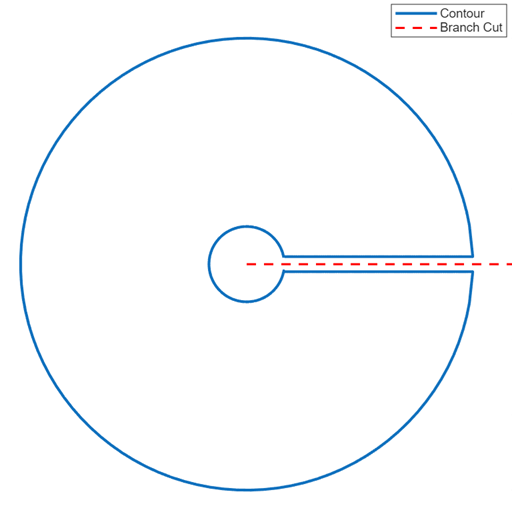
\includegraphics[scale=0.5]{Images/math555_keyhole.png}
   \end{center}

   In the limit, the two lines lie "along the branch cut" of $L$. This property can be exploited to effectively evaluate this integral. Consider the constituent parts of $\int_{\gamma_{r,R}}f(z)dz$. The keyhole contour has four parts: an inner contour of radius $r$, which contributes $-\int_{\partial \mathbb{D}_r}$, an outer contour of radius $R$ which contributes $\int_{\partial\mathbb{D}_R} f(z)dz$, and two lines along the real axis, which contribute: \begin{eqnarray*}
       \int_r^R \frac{L(z)}{(z+1)^2+4}dz - \int_r^R \frac{L(z)}{(z+1)^2+4}dz  \xrightarrow[\mathbb{H}_{-}\ni z\to t]{\mathbb{H}\ni z\to t} &&\int_r^R \frac{\log t + 0i}{(t+1)^2 + 4}dt -\int_r^R \frac{\log t + 2\pi i}{(t+1)^4 + 4}dt\\
       &=& -2\pi i\int_r^R \frac{1}{(t+1)^4+4}dt \\
       &=& -2 \pi i I_{r,R}\end{eqnarray*}
       Therefore, \[\int_{\gamma_{r,R}} f(z)dz = -2\pi i I_{r,R} - \int_{\partial \mathbb{D}_r} f(z)dz + \int_{\partial \mathbb{D}_R} f(z)dz\]

       Note that $\gamma_{r,R}$ encircles two singularities of $f$, namely $-1\pm 2i$. By the residue theorem, \begin{eqnarray*}
    \int_{\gamma_{r,R}} f(z)dz &=& 2\pi i \Res_{z=-1+2i} f(z) + 2\pi i \Res_{z=-1-2i} f(z)\\
    &=& 2\pi i \left[\Res_{-1+2i} \frac{L(z)}{(z+1)^2+4} + \Res_{-1-2i} \frac{L(z)}{(z+1)^2+4}\right]\\
    \text{(by pole formula)} &=& 2\pi i \left[\frac{L(-1+2i)}{(-1+2i)-(-1-2i)} + \frac{L(-1-2i)}{(-1-2i)-(-1+2i)}\right]\\
    &=& 2\pi i \frac{L(-1+2i)-L(-1-2i)}{4i}\\
    &=& \frac{\pi}{2} \bigg[\log \sqrt{5} + i\operatorname{HArg}(-1+2i) - \log \sqrt{5} - i\operatorname{HArg}(-1-2i)\bigg]\\
    &=& \frac{i\pi}{2} \left([\pi - \arctan(2)] - [\pi + \arctan(2)]\right)\\
    &=& - \pi i \arctan(2)
\end{eqnarray*} Now, the ML estimate will show that the remainder terms are zero. If $\rho>0$ and $\rho \neq 1$, we have: \[\left|\int_{\partial\mathbb{D}_\rho} f(z)dz\right| \leq 2\pi \rho \cdot \sup_{z\in \partial\mathbb{D}_\rho} \left|\frac{\log |z| + i\operatorname{HArg}z}{(z+1)^2+4}\right| \leq 2\pi \rho (\log |\rho|+ 2\pi) \sup_{z\in\partial\mathbb{D}_\rho} \left|\frac{1}{(z+1)^2 + 4}\right|\] If $\rho < 1$, then: \[2\pi \rho (\log |\rho|+ 2\pi) \sup_{z\in\partial\mathbb{D}_\rho} \left|\frac{1}{(z+1)^2 + 4}\right| \leq \frac{2\pi \rho (\log |\rho| + 2\pi)}{(\rho + 1)^2 + 4} = 2\pi \underbrace{\frac{\log |\rho^\rho| + 2\pi \rho}{(\rho+1)^2 + 4}}_{\rho < 1 \implies1/e\leq|\rho^\rho| < 1} < 2\pi \frac{1+2\pi \rho}{(\rho+1)^2+4} \xrightarrow[]{\rho \to 0} 0\] If $\rho>1$, then: \[2\pi \rho (\log |\rho|+ 2\pi) \sup_{z\in\partial\mathbb{D}_\rho} \left|\frac{1}{(z+1)^2 + 4}\right| \leq \underbrace{\frac{2\pi \rho\cdot (\rho^{1/2}+2\pi)}{(\rho+1)^2+4}}_{\log \rho < \sqrt{\rho}\text{ asymptotically}} \xrightarrow[]{\rho \to +\infty} 0\] Therefore, in the limit, both $\int_{\partial\mathbb{D}_r} f(z)dz \xrightarrow[]{r\to 0} 0$ and $\int_{\partial\mathbb{D}_R} f(z)dz \xrightarrow[]{R\to +\infty} 0$. Therefore, we have that: \[I = \lim_{(r,R)\to(0,+\infty)} I_{r,R} = -\frac{1}{2\pi i}\int_{\gamma_{r,R}} f(z)dz  = \frac{\pi i\arctan 2}{2\pi i} = \boxed{\frac{\arctan 2}{2}}\] This technique is often referred to as the "$\log$ trick," and it can be used to solve many similar integrals.
\end{framed}

A final result from the study of residues is presented for its utility. Its proof is not presented, as the material required is somewhat detached from the discussion of singularities.

\textbf{Rouche's Theorem}. Let $U\subseteq\mathbb{C}$ be an open set, and let $\gamma$ be a Jordan contour in $U$ such that the inside of $\gamma$ is fully contained in $U$. If $f,g:U\to\mathbb{C}$ are holomorphic and \[|g(z)-f(z)| < f(z)\] for all $z\in\gamma^*$ (i.e. \textit{along} the path of the contour), then $f$ and $g$ have the same number of zeros (counted with order) inside of $\gamma$.

Practically speaking, Rouche's theorem is a tool which allows one to count how many zeros occur within a given domain, which is generally not an obvious, by considering a more obvious function. Rouche's theorem is often utilized by selecting a function $f$ such that $\left|\frac{g(z)-f(z)}{f(z)}\right| < 1$, where $f$ is chosen so that the number of zeros of $f$ within the desired domain is immediately apparent.

\textbf{Example}. How many zeroes does the polynomial \[g(z) := z^6+9z^4+z^3+2z+4\] have on $\mathbb{D}$?

\textit{Solution}. It is obvious that $g$ has $6$ zeroes on the complex plane, but it is far from obvious how many lie within the unit disk in particular. However, by taking $f(z):=9z^4$, and considering the following quantity: \[\left|\frac{g(z)-f(z)}{f(z)}\right| = \left|\frac{z^6 + z^3 +2z +4}{9z^2}\right| \leq \left|\frac{z^4}{9}\right| + \left|\frac{z}{9}\right| + \left|\frac{2}{9z}\right| + \left|\frac{4}{9z^2}\right| \overset{z\in\partial\mathbb{D}}{=} \frac{1}{9} + \frac{1}{9} + \frac{2}{9} + \frac{4}{9} = \frac{8}{9}<1\] we see that Rouche's theorem applies, and $g$ has the same number of zeroes on $\mathbb{D}$ as $f$. Clearly, $9z^4$ has four zeroes (counted with order) at $z=0$, so $g$ has four zeroes on $\mathbb{D}$.

In principle, this result can be applied to \textit{any} function, not just polynomials.

\subsection{The Laplace Equation with Dirichlet Boundary Conditions}

Complex analysis can be applied to solve the Laplace Equation with Dirichlet boundary conditions. This particular partial differential equation comes up in several other areas. Notably, the Laplace equation is the heat equation $u_t = \alpha \nabla^2 u$ with $u_t\equiv 0$, i.e. at steady-state. Other examples emerge in fluid mechanics and electrodynamics. First, some definitions and properties are presented for a general class of functions called \textit{harmonic functions}.

\textbf{Definition}. Let $U\subseteq\mathbb{C}$ be open. Let $u:U\to\mathbb{C}$ be twice-differentiable on $U$. $U$ is called \textbf{harmonic} if \[\Delta u \equiv \nabla^2 u := \displaystyle\frac{\partial^2 u}{\partial x^2} +\frac{\partial^2 u}{\partial y^2} \equiv 0\]

Note that for any holomorphic $f:U\to\mathbb{C}$ where $f(z) = u(z) + i v(z)$, the Cauchy-Riemann equations give us that: \[\Delta u = \partial_1^2 u + \partial_2^2 u = \partial_1 \partial_2 v - \partial_2\partial_1 v = \underbrace{\partial_1\partial_2 v - \partial_1\partial_2 v}_\text{interchangeable order} = 0\] Therefore, the real part $u$ of $f$ is harmonic. Similarly, the imaginary part $v$ of $f$ is also harmonic. The functions $u$ and $v$ are called \textbf{harmonic conjugates} in $U$. This constitutes one simple way to check whether a function $u$ is harmonic: it suffices to show that $u$ is the real part (or the imaginary part) of a holomorphic function. 

Another method to find harmonic conjugates is by partial integration. In particular, suppose $u$ is a harmonic function. Then, the function $v$ must satisfy: \[v(x,y) = \begin{cases}
    \displaystyle\int \frac{\partial v(x,y)}{\partial y}dy = \displaystyle\int \frac{\partial u(x,y)}{\partial x} dy\\
    \displaystyle\int\frac{\partial v(x,y)}{\partial x}dx = -\displaystyle\int \frac{\partial u(x,y)}{\partial y}dx
\end{cases}\] where this relationship comes directly from integrating the Cauchy-Riemann equations.

Another property of harmonic functions is given, which also serves as an alternative characterization of harmonic functions.

\textbf{Mean value property for harmonic functions}. Let $U\subseteq\mathbb{C}$ be an open set, $z_0\in U$, and $R>0$ such that $\mathbb{D}_R(z_0)\subseteq U$. A function $u:U\to\mathbb{R}$ is harmonic if an only if it has the mean value property: \[u(z_0) = \frac{1}{2\pi r} \int_{\partial\mathbb{D}_r(z_0)} u(z)|dz| \ \ \ \forall r\in (0,R) \tag{Mean Value Property}\] This kind of integral is called an \textbf{arclength integral}, defined for any contour $\gamma:[a,b]\to\mathbb{C}$ and any function $g:\gamma^*\to \mathbb{C}$ to be the following complex number: \[\int_\gamma g(z)|dz| := \int_a^b g(\gamma(t)) |\gamma'(t)| dt\] Some additional properties will be outlined, which can be shown to follow quickly from each other.

\textbf{Identity Theorem for Harmonic Functions}. suppose $U\subseteq\mathbb{C}$ is a domain, and $u:U\to\mathbb{R}$ is harmonic. If there exists $z_0\in U$ and $r>0$ such that $\mathbb{D}_r(z_0)\subseteq U$ and $u$ is constant on $\mathbb{D}_r(z_0)$, then $u$ is constant on all of $U$.

Note that this result is much weaker than the identity theorem for analytic functions.

\textbf{Maximum and Minimum Principles with Boundary for Harmonic Functions}. Let $U\subseteq\mathbb{C}$ be a non-empty, bounded domain. If $u:\overline{U}\to\mathbb{R}$ is harmonic in $U$ and continuous in $\overline{U}$, then there exists a $z_0\in\partial U$ such that $u(z_0)=\max \{u(z)\mid z\in \overline{U}\}$ and a $z_1\in\partial U$ such that $u(z_1)\min\{u(z)\mid z\in\overline{U}\}$.

\begin{framed}
    \textbf{Statement of The Laplace Equation with Dirichlet Boundary Conditions}. Let $U\subseteq\mathbb{C}$ be an open set such that $\partial U \neq \varnothing$. Let $h:\partial U \to \mathbb{R}$. A function $u:U\to \mathbb{R}$ is a solution to the Laplace Equation with Dirichlet boundary condition $h$ if $u$ satisfies: 
        \[\Delta u \equiv 0\ \ \ \text{on }U \tag{Laplace's Equation}\]
        \[\displaystyle\lim_{U\ni z \to \zeta\in \partial U} u(z) = h(\zeta) \tag{Dirichlet BC}\] Note that the Laplace equation is precisely the statement that $u$ is harmonic, and the Dirichlet boundary condition is the statement that $u$ agrees with prescribed boundary data $h$.

        \textbf{Theorem} (Uniqueness of Solutions). If $U$ is bounded and $h:\partial U\to \mathbb{R}$ is continuous, then there exists at most one solution, $u$, to the Laplace equation on $U$ with Dirichlet boundary condition $h$.

        \begin{proof}
            Suppose $u_1,u_2:\overline{U}\to\mathbb{R}$ are two solutions to the Laplace equation with Dirichlet boundary data $h$. Since $u_1$ and $u_2$ are complex differentiable, $u_1$ and $u_2$ are continuous. Also note that $u_1=h=u_2$ on $\partial U$. We show a corollary.

            \textbf{Corollary}. Suppose $U\subseteq\mathbb{C}$ is a nonempty bounded domain. Suppose $u_1,u_2:\overline{U}\to\mathbb{R}$ are harmonic in $U$ and continuous in $\overline{U}$. If $u_1=u_2$ on $\partial U$, then $u_1=u_2$ on all of $\overline{U}$.

            \textit{Proof of the Corollary}. Define $u:= u_1-u_2$. Note that $u$ is harmonic in $U$ and continuous in $\overline{U}$. By the maximum and minimum principle with boundary, there exists $z_0,z_1\in U$ such that \[\max_{z\in\overline{U}} u(z) = u(z_0)= 0 = u(z_1)=\min_{z\in\overline{U}} u(z_1)\] which implies that $u$ is constant.

            With the corollary, $u_1=u_2$ on $\overline{U}$.
        \end{proof}

        A discussion of existence is much more complicated, but one set for which a solution always exists is on closed disks.

        \textbf{Theorem} (Existence of Solutions on Disks). Define the \textit{Poisson kernel} for all $z,\zeta\in\mathbb{C}$, $z\neq \zeta$ as follows: \[P(z,\zeta) := \frac{|\zeta|^2-|z|^2}{|z-\zeta|^2}\] Let $R>0$, and let $h:\partial\mathbb{D}_R$ be continuous. The function $u:\overline{\mathbb{D}}_R\to\mathbb{R}$ defined by: \[u:=\frac{1}{2\pi R} \int_{\partial\mathbb{D}_R} h(z)P(z,\zeta)|d\zeta|\tag{Poisson's Integral Formula}\] is a solution to the Laplace Equation on $\mathbb{D}_R$ with Dirichlet boundary data $h$.

        The arclength integral which gives $u$ is called \textit{Poisson's integral formula}. The proof that $u$ is harmonic is relatively straightforward, with one only needing to show that $u$ is the real part of a differentiable function. It is much more challenging to show that $u(z)\to h(\zeta)$ as $\mathbb{D}_R\ni z\to \zeta\in \partial \mathbb{D}_R$, but it is true.
\end{framed}

The disk is not the only domain on which the Laplace equation can be solved subject to Dirichlet boundary conditions. Solutions can be transformed between topologically equivalent sets by constructing a suitably well-behaved map (i.e. a homeomorphism). Let $S\subseteq\mathbb{C}$. Define $\operatorname{cl}_\infty (S)$ to be the closure of $S$ in $\hat{\mathbb{C}}$, and let $\partial_\infty S$ be the boundary of $S$ in $\hat{\mathbb{C}}$; namely, if $S$ is bounded, then $\operatorname{cl}_\infty (S) = \overline{S}$ and $\partial_\infty S = \partial S$, and if $S$ is unbounded this set includes $\infty$.

\textbf{Definition}. Let $U,V\subseteq\mathbb{C}$ be domains. A \textbf{Riemann map} from $U$ to $V$ is a homeomorphism $\Phi:\operatorname{cl}_\infty(U)\to \operatorname{cl}_\infty(V)$ such that $\Phi(\partial_\infty U) = \partial_\infty V$.

\textbf{Definition}. A bounded subset $\Omega\subseteq \mathbb{C}$ is called a \textbf{Jordan domain} if there exists a Jordan curve $\gamma$ such that $\Omega$ is the set of points enclosed by $\gamma$.

\textbf{Theorem} (Riemann Mapping Theorem). Suppose $\Omega\subseteq\mathbb{C}$ is a Jordan domain. Then, there exists a Riemann map from $\Omega$ to $\mathbb{D}$. In addition, if $z_1,z_2,z_3\in\partial\Omega$ are distinct points (oriented counterclockwise), and $w_1,w_2,w_3\in\partial \mathbb{D}$ are distinct points (oriented counterclockwise), then there exists a unique Riemann map $\Phi : \overline{\Omega}\to\overline{\mathbb{D}}$ such that $\Phi(z_i)=w_i$.

The proof of the Riemann mapping theorem is outside the scope of this material, but it can be used to guarantee solutions exist on Jordan domains. Since a Riemann map is guaranteed to exist, 

\begin{framed}
\textbf{Theorem} (Existence of Solutions on Jordan Domains). Suppose $\Omega\subseteq\mathbb{C}$ is a Jordan domain, and let $h:\partial\Omega\to \mathbb{R}$ be continuous Dirichlet boundary data. Choose a Riemann map $\Phi$ from $\Omega$ to $\mathbb{D}$ (which exists by the Riemann mapping theorem), and define \[h_\mathbb{D}(z) := h(\Phi^{-1}(z))\ \ \ \forall z\in\partial\mathbb{D}\] If $u_\mathbb{D}$ is a solution to the Laplace equation on $\mathbb{D}$ with Dirichlet boundary data $h_\mathbb{D}$ (given by Poisson's integral formula), then the function \[u:=u_\mathbb{D}\circ \Phi\] is a solution to the Laplace equation on $\Omega$ with Dirichlet boundary condition $h$.
\end{framed}

The only question, then, is how to construct Riemann maps. This can be done by studying a well-behaved class of conformal maps called \textbf{fractional linear transformations} (FLTs). For the following discussion, let $A$ be a matrix of the form $A:=\begin{bmatrix}
    a & b\\
    c & d
\end{bmatrix}$ where $a,b,c,d\in\mathbb{C}$ and $\det A \neq 0$, i.e. $A$ is invertible, and its inverse is given by $A^{-1} = \frac{1}{ad-bc}\begin{bmatrix}
    d & -b\\
    -c & a
\end{bmatrix}$

The fractional linear transformation associated with $A$ is the map $T_A:\hat{\mathbb{C}}\to\hat{\mathbb{C}}$ defined by: \[T_A(z) := \frac{az+b}{cz+d}\] with the convention that $\frac{1}{\infty} = 0$, $\frac{1}{0}=\infty$, and $\frac{\infty}{\infty} = 1$. Some nice properties follow, which are immediately obvious (outside of the mentioned edge-cases, in which case the results can be shown by applying the conventions): $T_A$ is a continuous map, $T_A\circ T_B= T_{AB}$, and $T_A=T_B\iff A=c B$ for some $c\in\mathbb{C}\setminus\{0\}$. 

Perhaps the most important property, which motivates the study of FLTs at all, is that $T_A$ is a homeomorphism with $T_A^{-1} = T_{A^{-1}}$. Namely, $T_A$ is simple to invert, and $T_A$ acts as a conformal map between two subsets of $\hat{\mathbb{C}}$. Another key result which is much less obvious is that FLTs which share three points are identical.

\textbf{Uniqueness Property of FLTs}. Let $A,B$ be matrices as above. Let $z_1,z_2,z_3\in\hat{\mathbb{C}}$ such that $T_A(z_i) = T_B(z_i)$ for all $i\in\{1,2,3\}$. Then, $T_A=T_B$, i.e. $A=cB$ for some $c\neq 0$. That is, if two FLTs agree at three points, they are the same FLT.

This fact allows the construction of FLTs by assigning a mapping to only three points.

\begin{shaded}
    \textbf{Construction of FLTs}. Let $(z_1,z_2,z_3)$ be distinct and $(w_1,w_2,w_3)$ be distinct. The following discussion will provide a guide for constructing an FLT from $(z_1,z_2,z_3)$ to $(w_1,w_2,w_3)$, and therefore for constructing an FLT between any two spaces.

    \textbf{Definition}. Let $z\in \hat{\mathbb{C}}$, and consider four points $(z_0,z_1,z_2,z_3)$. The \textbf{cross-ratio} is defined as the quantity \[[z_0,z_1,z_2,z_3] := \frac{z_0-z_1}{z_0-z_3} \frac{z_2-z_3}{z_2-z_1}\]

    If $(z_1,z_2,z_3)$ is a collection of distinct points, this is an FLT, i.e. the map \[z\mapsto [z,z_1,z_2,z_3] = \frac{z-z_1}{z-z_3} \frac{z_2-z_3}{z_2-z_1}\] is an FLT (note that the quantity $\frac{z_2-z_3}{z_2-z_1}$ is a constant). Note in particular that $F(z_1) = 0$, $F(z_2) = 1$, and $F(z_3)=\infty$, i.e. $F$ maps the triplet $(z_1,z_2,z_3)$ to the triplet $(0,1,\infty)$. This very specific FLT can be used to construct \textit{any} FLT between triplets of points, as the following discussion shows.

    Consider the FLTs defined by $F(z):=(z,z_1,z_2,z_3)$, and $G(z):=[w,w_1,w_2,w_3]$. Then, note that: \[\begin{bmatrix}
        z_1\\
        z_2\\
        z_3
    \end{bmatrix} \overset{F}{\longrightarrow} \begin{bmatrix}
        0\\
        1\\
        \infty
    \end{bmatrix}\overset{G}{\longleftarrow}\begin{bmatrix}
        w_1\\
        w_2\\
        w_3
    \end{bmatrix}\] Therefore, \[\begin{bmatrix}
        z_1\\
        z_2\\
        z_3
    \end{bmatrix} \overset{F}{\longrightarrow} \begin{bmatrix}
        0\\
        1\\
        \infty
    \end{bmatrix} \overset{G^{-1}}{\longrightarrow} \begin{bmatrix}
        w_1\\
        w_2\\
        w_3
    \end{bmatrix} \Longrightarrow \begin{bmatrix}
        z_1\\
        z_2\\
        z_3
    \end{bmatrix} \xrightarrow[]{F\circ G^{-1}} \begin{bmatrix}
        w_1\\
        w_2\\
        w_3
    \end{bmatrix}\] This shows that an FLT can be constructed in general between any two triplets of distinct points. Specific steps are as follows: \vspace{-1em}\begin{enumerate}
        \item[1.] Define $T_A := [z,z_1,z_2,z_3]$, i.e. an FLT from $(z_1,z_2,z_3)$ to $(0,1,\infty)$.
        \item[2.] Define $T_B:= [w,w_1,w_2,w_3]$, i.e. an FLT from $(w_1,w_2,w_3)$ to $(0,1,\infty)$.
        \item[3.] Compute $B^{-1}$, which is simple for a $2\times 2$ matrix.
        \item[4.] Compute $T_A\circ T_B^{-1} = T_{AB^{-1}}$, i.e. multiply $AB^{-1}$ and construct the FLT from the resulting transformation.
    \end{enumerate}

    An important fact allows one to construct FLTs which map desired sets under certain conditions, rather than just three points.

    \textbf{Definition}. A set $C\subseteq\hat{\mathbb{C}}$ is a \textbf{generalized circle} if $C$ is a circle (i.e. the boundary of some disk in $\mathbb{C}$) or if $C=L\cup \{\infty\}$ for some line $L\subseteq\mathbb{C}$.

    This definition makes sense if one considers the limiting case of a circle, where the radius is infinitely large and becomes, in the limit, a perfect line dividing the plane in two.

    \textbf{Fact}. A generalized circle has two sides: an inside, and an outside. If $C$ is a true circle, the inside of $C$ is the inside of the circle, and the outside is the rest of $\hat{\mathbb{C}}$; if $C$ is a line, the inside is one half of the plane (not including $\infty$), and the outside is the rest of $\hat{\mathbb{C}}$, i.e. including $\infty$. In either case, the sides of $C$ are nonempty, disjoint, connected sets $S_1,S_2\subseteq\hat{\mathbb{C}}$ such that $\hat{\mathbb{C}}\setminus C = S_1\cup S_2$, i.e. $C$ separates the extended complex plane into two pieces.

    \textbf{Theorem} (Action of FLTs on Generalized Circles). Suppose $F:\hat{\mathbb{C}} \to \hat{\mathbb{C}}$ is an FLT and $C\subseteq\hat{\mathbb{C}}$ is a generalized circle with sides $S_1$ and $S_2$. Then, the image $F(C)\subseteq\hat{\mathbb{C}}$ is a generalized circle with sides $F(S_1)$ and $F(S_2)$.

    This theorem is somewhat painful to prove, but not particularly surprising; note that FLTs are constructed in such a way as to be homeomorphisms, i.e. mappings which preserve topology. It is therefore natural that this fundamental aspect of the topology of generalized circles, i.e. that they have a connected inside and a connected outside, is preserved. Regardless, this fact allows one to determine how an FLT maps sets by checking (or assigning, through an FLT) only three points on the boundary and one point on the inside or outside.
\end{shaded}

\textbf{Example}. Construct an FLT from $\mathbb{D}$ to the upper-half plane $\mathbb{H}$.

\textit{Solution}.  We will map $\partial \mathbb{D}$ to $\mathbb{R}=\partial\mathbb{H}$, then use the theorem about the action of FLTs on generalized circles to deduce which side of the circle gets mapped to where, and apply a rotation if necessary. Let us try mapping $(1,i,-1)\to (0, 1, \infty)$. Define: \[T_A = [z, 1, i, -1] = \frac{z-1}{z+1} \frac{i+1}{i-1} = -i\frac{z-1}{z+1} \implies A = -i\begin{bmatrix}
    1 & -1\\
    1 & 1
\end{bmatrix}\] Then, define: \[T_B = [z,0,1,\infty] = \frac{z-0}{z-\infty} \frac{1-\infty}{1-0} = \frac{z}{1} \implies \begin{bmatrix}
    1 & 0\\
    0 & 1
\end{bmatrix}\] Clearly, $B=I_2$ is its own inverse, and it is the identity, which means that: \[F:=T_{AB^{-1}} = T_A = -i \frac{z-1}{z+1}\] is an FLT mapping $\partial\mathbb{D}$ to $\mathbb{R}$. Now, we use the fact that $\mathbb{R}$ and $\partial\mathbb{D}$ are generalized circles and investigate which side of $\partial\mathbb{D}$ maps to which side of $\mathbb{R}$. Since $0\in\partial\mathbb{D}$, i.e. $0$ is on the inside of $\partial\mathbb{D}$, it suffices to check this point. Note that: \[F(0) = -i\frac{0-1}{0+1} = i \in\mathbb{H}\]

As an aside, the fact that there is a Riemann map from $\overline{\mathbb{D}}$ to $\overline{\mathbb{H}}$, i.e. the mapping $F$ which was just found, implies that the Laplace Equation can be solved subject to Dirichlet boundary conditions on $\mathbb{H}$. The exact form of the solution can be found through some (fairly painful) algebra.

\textbf{Theorem} (Existence of Solutions in the Upper-Half Plane). Suppose $h:\mathbb{R}\to\mathbb{R}$ is a continuous function such that \[h_\infty := \lim_{\mathbb{R}\ni x\to +\infty} h(x) = \lim_{\mathbb{R}\ni x\to -\infty} h(x) \in \mathbb{R}\] Then, there exists a solution $u$ to the Laplace equation on $\mathbb{H}$ subject to boundary data $h$, given by \[u(x,y) = \frac{y}{\pi} \int_{-\infty}^{+\infty} \frac{h(t)}{(t-x)^2 + y^2} dt\ \ \ \ \ \ \ \ \text{where }(x,y)\in\mathbb{H}\]

This follows from transforming the formula which solves the Laplace equation on $\mathbb{D}$ via the above FLT.